\chapter{讨价还价} \label{ch11:chap11}

本章旨在阐述讨价还价模型。现实生活中，房屋买卖双方之间的互动即为一个讨价还价的案例。这属于一个博弈论问题，因为在这一过程中，考量对手的处境至关重要。若能达成协议，博弈双方均可从中获益。

一个基本的讨价还价模型是“分蛋糕”模型，要以双方都能接受的方式进行分配，但在这个范围内，一方的收益必然意味着另一方的损失，核心问题在于如何实现公平分配。约翰·纳什在其本科毕业论文（后发表于Nash （1950））中，提出了一套公理，即通过若干自然条件推导出公平的“讨价还价解”。纳什证明，这些公理总能得出唯一解，而且这个解也很容易计算。第~\ref{sec11.2}~节展示了如何从双矩阵博弈(这里是囚徒困境的一个变体)中推导出讨价还价集，在这个博弈中，玩家可以从合作中受益。第~\ref{sec11.3}~节和第~\ref{sec11.4}~节介绍了一般的讨价还价集和相应的公理，第~\ref{sec11.5}~节对讨价还价解进行了几何刻画。

纳什讨价还价模型并非我们此前探讨的策略式或扩展式非合作博弈，而是属于\textit{合作博弈}理论，该理论假设玩家能够以某种方式达成协议并共同遵守。模型描述了可能达成的协议及其收益分配机制，但既未说明促成协议的具体行动细节，也未涉及协议的执行保障。合作博弈论的典型方法是提出博弈的\textit{解}（理想情况下为唯一解，例如达成某项特定协议），且这些解必须满足特定的\textit{公理}。而纳什讨价还价解正是这类解决方案的典型代表。

本章后面的章节回到了鲁宾斯坦(Rubinstein，1982)提出的非合作讨价还价模型。该模型使用具有完美信息的博弈树，玩家轮流提出报价，另一方可以接受或拒绝。对这个博弈的分析运用了第~\ref{sec-4.7}~节所述的承诺博弈理论。最基本的形式是第~\ref{sec11.7}~节介绍的最后通牒博弈：一方提出单一报价，另一方只能选择接受或拒绝。

在第~\ref{sec11.8}~节和第~\ref{sec11.9}~节描述的多轮交替报价博弈中，每一轮都有可能因为双方无法达成协议而导致博弈无法进入下一轮，最终双方一无所获。这产生了一个“贴现因子”，它量化了早期协议相较于延迟协议的优势程度。参与人通过前瞻推演，其最优策略形成一系列交替出价序列，并在首轮达成协议。这种策略既适用于固定轮次谈判，也可采用“平稳策略”处理无限轮次讨价还价。本质上，当轮到同一玩家报价时，博弈每两轮重复一次（见第~\ref{sec11.10}~节）。第~\ref{sec11.11}~节展示了交替报价讨价还价模型得出的一个精妙结论：当贴现因子体现参与人极具耐心时，博弈均衡结果与纳什公理化讨价还价解\textit{一致}。由此，基于自利行为构建的模型为纳什合作式解的概念提供了理论支撑。


\section{预备知识和学习目标}\label{sec11.1}

本章的预备知识包括:策略式两人博弈(第~\ref{c3}~章)、效用函数允许正仿射变换的概念(第~\ref{sec:5.6}~节)、凹效用函数(第~\ref{sec:5.9}~节)、承诺博弈(第~\ref{sec-4.7}~节)和极大极小策略(第~\ref{sec:8.2}~节)。

学习本章后，你应该能够:
\begin{itemize}
\item 解释讨价还价集、讨价还价公理、纳什讨价还价解、威胁点和纳什积的概念；
\item 绘制从双矩阵博弈导出的讨价还价集，以及当玩家具有凹效用函数时对“单位蛋糕”进行讨价还价的讨价还价集；
\item 解释并解决多轮出价与反出价议价模型的具体例子，以及无限轮次的平稳子博弈完美均衡。
\end{itemize}

\section{讨价还价集}\label{sec11.2}

考虑图~\ref{fig:11.1}左侧所示的囚徒困境博弈变体。参与人I的策略$B$严格占优于$T$，参与人II的策略$r$严格占优于$l$，因此该博弈唯一纳什均衡为$(B,r)$，两名参与人的收益均为$1$。反观策略组合$(T,l)$，参与人I、参与人II可分别获得收益$2$与$3$，该结果能同时提升双方福利，显然更帕累托占优。

现在假设玩家可以相互交流，并就他们打算遵循的某种行动方案达成了一致。我们不建模玩家如何交流、达成协议或执行他们的协议，而是试图给出他们应该达成何种协议的指导原则。

第一步是通过描述一个可协商的“讨价还价集"来建模玩家通过协议所能达成的结果，该集合包含所有可能实现的收益对组合。假设玩家可以就图~\ref{fig:11.1}收益表中的任何单元格的策略达成一致。由此产生的效用对$(u,v)$是二维图中的点，其中横坐标\(u\) 代表玩家I的效用，纵坐标\(v\) 代表玩家II的效用。这些点已标注在图~\ref{fig:11.1}右侧，并附有对应的策略组合标记。例如标注为 \(T,l\)的点对应效用对$(2,3)$。

\begin{figure}[htbp]
\centering
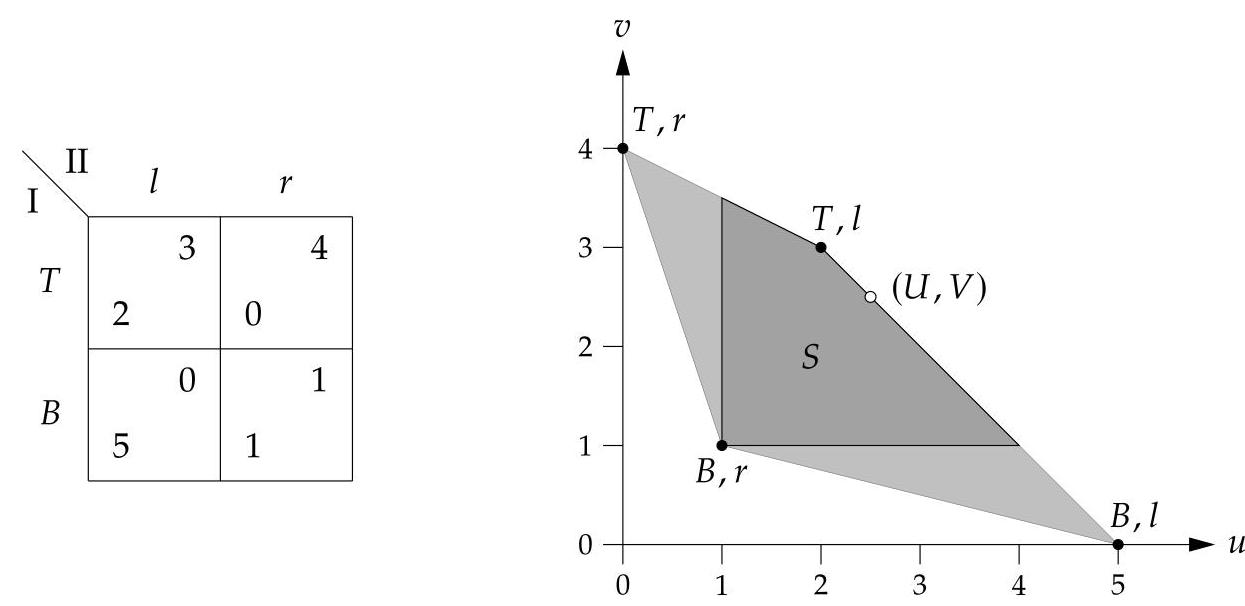
\includegraphics[width=0.9\textwidth]{translation/images/ch11-fig01.jpg}
\caption{左侧: \(2 \times  2\) 类似于囚徒困境的博弈。右侧:相应的讨价还价集 \(S\) (深灰色)及其讨价还价解$(U,V)$。}
\label{fig:11.1}
\end{figure}

这些效用对的凸包(凸组合的集合)在图~\ref{fig:11.1}中以浅灰色和深灰色显示。任何此类凸组合，均可通过参与者基于协议约定、决定采用的联合抽签方式得到。例如，如果玩家决定抛一枚硬币，并根据结果选择$(T,l)$或$(B,r)$，那么效用对$(1.5,2)$将是期望效用。我们假设这次抛硬币以及随后的联合行动是玩家协议的一部分，并且他们会执行该协议。

借助抽签机制使讨价还价集成为凸集并不像听起来那么奇怪。例如，当两人都希望获得某件不可分割的物品时，抛硬币决定归属权通常被视为一种公平的解决方案。

并非凸集合中的每个点都是“合理的”，因为我们始终假定参与者有权提前拒绝接受该点对应的方案。例如，玩家I不会同意两个玩家确定地选择策略对$(T,r)$，在这种情况下玩家I的收益为零。究其原因，即便不存在任何协议，玩家I也可以使用他的极大极小策略 \(B\)，无论另一个玩家做什么，该策略都能保证他获得1的收益。正如第~\ref{c8}~章零和博弈所述，极大极小策略可能是一种混合策略；但在图~\ref{fig:11.1}的囚徒困境博弈中，它是一种纯策略。我们要求：议价情境下所有达成一致的结果，必须保证每位参与人至少获得其极大极小收益（通常根据该玩家自己的收益来定义）。

因此，从策略形式的两人博弈中导出的讨价还价集 \(S\) 被定义为效用对的凸包（如博弈中所指定），并附加约束条件:对于 \(S\) 中的所有$(u,v)$，有 \(u \geq  {u}_{0}\) 和 \(v \geq  {v}_{0}\)，其中 \({u}_{0}\) 是玩家I的极大极小收益， \({v}_{0}\) 是玩家II的极大极小收益。当 \({u}_{0} = {v}_{0} = 1\)时，最终形成的集合 \(S\) 在图~\ref{fig:11.1}中以深灰色显示。

在这个例子中，“纳什讨价还价解”（不要将其与“纳什均衡”相混淆，这是一个截然不同的概念）将给出效用对 \(\left( {U,V}\right)  = \left( {{2.5},{2.5}}\right)\)，下文将对此展开推导（ \(U = V\) 只是巧合）。这个期望效用对是效用对 $(2,3)$ 和 $(5,0)$ 的凸组合。它是通过一个联合抽签机制实现的，该抽签机制以概率 \(\frac{5}{6}\) 选择 $(T,l)$，以概率 \(\frac{1}{6}\) 选择 $(B,l)$。实际上，玩家 II 总是选择 \(l\)，而玩家 I 以概率 \(\frac{5}{6}\) 和 \(\frac{1}{6}\) 在 \(T\) 和 \(B\) 之间进行选择。然而，这不是混合策略，而是由一个独立设备进行的抽签机制，其结果是两个玩家事先就决定接受的。



\section{讨价还价公理}\label{sec11.3}

我们将讨价还价情形建模为讨价还价集，并尝试为任何此类情形找到一个解。关于这个模型的条件被称为公理，它们既涉及讨价还价集，也涉及我们想要得到的解。

\begin{definition}[讨价还价集的公理]\label{def:11.1}
具有威胁点 \(\left( {{u}_{0},{v}_{0}}\right)\) 的讨价还价集 \(S\) 是 \({\mathbb{R}}^{2}\) 的一个非空子集，使得

(a) 对于所有 \(\left( {u,v}\right)  \in  S\),有 \(u \geq  {u}_{0},v \geq  {v}_{0}\);

(b) \(S\) 是紧致的;

(c) \(S\) 是凸的。
\end{definition}

讨价还价集 \(S\) 中的每一对 $(u, v)$ 代表玩家 \(\mathrm{I}\) 的效用 \(u\) 和玩家 II 的效用 \(v\) ，玩家们可以通过达成特定协议来实现这些效用。因为 \(S\) 是非空的，所以至少有一种协议是可能的。威胁点 \(\left( {{u}_{0},{v}_{0}}\right)\) 是每个玩家(在期望意义上)可以为自己保底的效用对。定义~\ref{def:11.1} 中的公理 (b) 表明 \(S\) 是有界且闭的，其目的是通过某种最大化过程来定义一个讨价还价解。凸性公理 (c) 意味着，必要时玩家可以将联合抽签机制作为协议组成部分。

在第~\ref{sec11.2}~节中，我们基于一个双矩阵博弈 $(A,B)$ 构建了一个讨价还价集 \(S\) 并证明这个集合满足定义~\ref{def:11.1} 中的公理。其中公理 (b) 和 (c) 的成立是显而易见的。公理(a)虽直接成立，但我们必须证明 \(S\) 是非空的。威胁点 \(\left( {{u}_{0},{v}_{0}}\right)\) 的取值规则如下： \({u}_{0}\) 是玩家 I 的极大极小收益(基于其自身的收益函数)， \({v}_{0}\) 是玩家 II 的极大极小收益(基于其自身的收益函数)。因此，如果玩家 I 采用他的极大极小策略 \(\widehat{x}\)，玩家 II 采用他的极大极小策略 \(\widehat{y}\)，那么博弈中得到的收益组合 \(\left( {u,v}\right)  = \left( {{\widehat{x}}^{\top }A\widehat{y},{\widehat{x}}^{\top }B\widehat{y}}\right)\) 是 \(S\) 的一个元素，因为 \(u \geq  {u}_{0}\) 和 \(v \geq  {v}_{0}\)，所以 \(S\) 是非空的。

然而，在从双矩阵博弈构建讨价还价集时，威胁点 \(\left( {{u}_{0},{v}_{0}}\right)\) 本身不必是 \(S\) 的元素，如练习~\ref{exer:11.2}(ii)所示。出于这个原因，威胁点 \(\left( {{u}_{0},{v}_{0}}\right)\) 会与讨价还价集一起明确给出。如果威胁点属于 \(S\) 且条件(a)成立，那么就不可能有其他威胁点。如果威胁点包含在 \(S\) 中，下面定义~\ref{def:11.2}中的公理表述起来会更简单，但那样我们就必须采取额外的步骤才能从双矩阵博弈中得到这样一个讨价还价集。在我们的示例和图示中，我们通常会考虑包含威胁点的集合 \(S\) 。

此后，我们简单地假设讨价还价集 \(S\) 满足这些公理。后续我们将探讨适用于其他情形的讨价还价集，这类讨价还价集是被直接定义的，而非源于双矩阵博弈。

在下面的定义中，公理(d) - (h)是定义~\ref{def:11.1}中(a) - (c)的延续。我们随后会对它们进行讨论。

\begin{definition}[讨价还价解的公理]\label{def:11.2}
对于给定的具有威胁点 \(\left( {{u}_{0},{v}_{0}}\right)\) 的讨价还价集 \(S\)，讨价还价解 \(N\left( S\right)\) 是一个二元组$(U,V)$，使得

(d) \(\left( {U,V}\right)  \in  S\);

(e) 解$(U, V)$是帕累托最优的，即对于所有 \(\left( {u,v}\right)  \in  S\)，如果 \(u \geq  U\) 且 \(v \geq  V\)，那么 \(\left( {u,v}\right)  = \left( {U,V}\right)\)；

(f) 它具有效用缩放不变性，即如果 \(a,c > 0\) 且 \(b,d \in  \mathbb{R}\),并且 \({S}^{\prime }\) 是有威胁点 \(\left( {a{u}_{0} + b,c{v}_{0} + d}\right)\) 的讨价还价集 \(\{ \left( {{au} + b,{cv} + d}\right)  \mid  \left( {u,v}\right)  \in  S\}\),那么 \(N\left( {S}^{\prime }\right)  = \left( {{aU} + b,{cV} + d}\right)\);

(g) 它具有对称性，即如果 \({u}_{0} = {v}_{0}\) 且 \(\left( {u,v}\right)  \in  S\) 意味着 \(\left( {v,u}\right)  \in  S\)，那么 \(U = V\);

(h) 它满足无关选择独立性:如果 \(S,T\) 是具有相同威胁点的讨价还价集，且 \(S \subset  T\)，那么要么 \(N\left( T\right)  \notin  S\)，要么 \(N\left( T\right)  = N\left( S\right)\)。
\end{definition}

符号 \(N\left( S\right)\) 是“纳什讨价还价解”的简写。根据公理(d)，该解是属于讨价还价集 \(S\) 的两个参与者的效用二元组(U, V)。

(e)中所述的帕累托最优意味着，不可能在不损害另一个参与者的情况下改善一个参与者的解。因此，从图上看，解位于讨价还价集的右上边界（或“东北”）边界上，该边界也称为该集合的帕累托前沿。

(f)中所述的效用缩放不变性意味着，玩家的效用函数可以通过改变其“刻度”和“原点”来改变，而不改变其含义，就像温度刻度一样（见第~\ref{c5}~章）。对于玩家I，这样的变换是将原有效用 \(u\)替换为 \({au} + b\)，其中 \(a\) 和 \(b\) 是常数实数，且 \(a > 0\)。同理，对于玩家II，我们可以将\(v\)替换为\({cv} + d\)，其中 \(c,d\) 是常数实数，且 \(c > 0\)。在绘制讨价还价集 \(S\) 时，该变换的几何意义为，通过加上 \(b\)，该集合中任何点的横坐标整体平移\(b\)个单位(根据 \(b\) 的正负向右或向左移动)；并按系数\(a\)伸缩（\(a > 1\)拉伸\(a < 1\)收缩）。在条件(f)中，新谈判集合\({S}^{\prime }\) 和新的威胁点就是通过对两个玩家应用这样的“刻度变化”，后从原集合\(S\)变换得到的。

因为这种缩放不会改变效用值的含义（它们仍然代表相同的偏好），所以如公理(f)所述，讨价还价解也不应受到影响。从某种意义上说，这意味着讨价还价解不应依赖于对玩家效用的直接比较。例如，如果你想和一个朋友分一块巧克力，你不能因为你比她喜欢巧克力多十倍，就要求多分（你可以通过将你的效用从 \(u\) 改变为 \({10u}\) 来表示），她也不能因为你抽屉里已经有5块巧克力就要求你少分（通过从 \(u\) 改变为 \(u + 5\) 来表示）。

(g)中所述的对称性意味着，一个对称的讨价还价集 \(S\) （对于所有的$(u, v)$，我们有 \(\left( {u,v}\right)  \in  S \Leftrightarrow  \left( {v,u}\right)  \in  S\)），且威胁点的形式为 \(\left( {{u}_{0},{u}_{0}}\right)\)，其讨价还价解的形式也应该为 \(N\left( S\right)  = \left( {U,U}\right)\)。

（h）中所述的无关选择独立性是最复杂的公理。如图~\ref{fig:11.2}所示，该公理的内涵为：若议价集$S$被扩展为一个包含新增效用组合$(u, v)$的更大集合$T$，且威胁点保持不变，则两种情况必居其一——要么集合$T$的议价解$N(T)$是某一新增效用组合，要么其议价解与原集合$S$的议价解$N(S)$完全相同。绝不允许出现这样的情况：集合$T$的议价解落到原集合$S$内的某一其他点上（例如图~\ref{fig:11.2}中的点$P$）。

\begin{figure}[htbp]
\centering
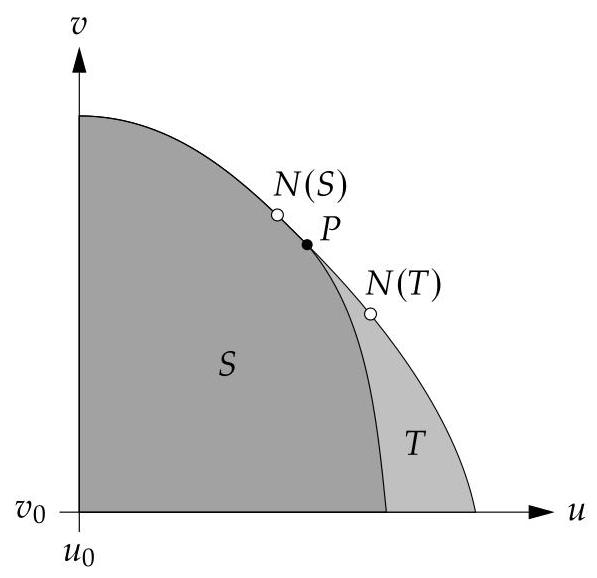
\includegraphics[width=0.4\textwidth]{translation/images/ch11-fig02.jpg}
\caption{讨价还价集 \(S\) (深灰色)和 \(T\) (深灰色和浅灰色)。无关选择独立性表明，如果 \(S\) 是 \(T\) 的子集，那么 \(N\left( T\right)\) 要么不在 \(S\) 中，就像这里一样，要么等于 \(N\left( S\right)\) ，但不能是 \(S\) 中的另一个点，如 \(P\) 。}
\label{fig:11.2}
\end{figure}

所陈述的讨价还价集和可能的讨价还价解的公理(a)-(h)是合理的要求，可以作为一般原则。


\section{纳什讨价还价解}\label{sec11.4}


本节表明，定义~\ref{def:11.1}和~\ref{def:11.2}中的讨价还价公理(a)--(h)意味着存在一个讨价还价解，而且这个解是唯一的。

\begin{theorem}\label{theo:11.3}
在纳什讨价还价公理下，每个包含点$(u,v)$且 \(u > {u}_{0}\) 和 \(v > {v}_{0}\) 的讨价还价集 \(S\) 都有一个唯一的解 \(N\left( S\right)  = \left( {U,V}\right)\)，该解是使乘积\(\left( {u - {u}_{0}}\right) \left( {v - {v}_{0}}\right)\) （也称为“纳什乘积”）在 \(\left( {u,v}\right)  \in  S\) 时达到最大值的唯一的点$(u,v)$。
\end{theorem}

\begin{proof}
首先，定义集合 \({S}^{\prime } = \left\{  {\left( {u - {u}_{0},v - {v}_{0}}\right)  \mid  \left( {u,v}\right)  \in  S}\right\}\)，该集合是将原谈判集\(S\) 经过平移后得到的，使得威胁点 \(\left( {{u}_{0},{v}_{0}}\right)\) 平移至坐标原点$(0,0)$，如图~\ref{fig:11.3} (a)和(b)所示。此时最大化纳什积就相当于在 \(\left( {u,v}\right)  \in  {S}^{\prime }\) 的条件下最大化 \({uv}\)。设$(U,V)$为取到该最大值的效用组合，根据前提假设满足 \({UV} > 0\)；图~\ref{fig:11.3} (b) 画出了双曲线 \({uv} = c\)，其中\(c\) 为能让该双曲线与集合 \({S}^{\prime }\)依旧存在交点的最大常数。接下来，我们对效用进行重新缩放，使得 \(\left( {U,V}\right)  = \left( {1,1}\right)\)，方法是构造新集合 \({S}^{\prime \prime } = \left\{  {\left. \left( {\frac{1}{U}u,\frac{1}{V}v}\right) \right| \;\left( {u,v}\right)  \in  {S}^{\prime }}\right\}\) 替换 \(S\)，如图~\ref{fig:11.3}(c)所示。为简化符号，我们将 \({S}^{\prime \prime }\) 重命名为 \(S\)。

接下来，定义集合 \(T = \{ \left( {u,v}\right)  \mid  u \geq  0,v \geq  0,u + v \leq  2\}\) ，见图~\ref{fig:11.3}(d)。对于讨价还价集 \(T\)，其纳什解为 \(N\left( T\right)  = \left( {1,1}\right)\)，原因是集合\(T\)具有对称性，并且(1,1)是 \(T\) 的帕累托前沿上唯一的对称点。我们可以证明 \(S \subseteq  T\)，又因为 \(N\left( T\right)  = \left( {1,1}\right)  \in  S\)，因此根据无关选项独立性公理，可推出 \(N\left( S\right)  = N\left( T\right)\)。

我们利用集合 \(S\) 的凸性来证明 \(S \subseteq  T\)。采用反证法，假设存在一个点 \(\left( {\bar{u},\bar{v}}\right)\) 属于集合 \(S\) ，但不属于集合 \(T\)。已知\(\bar{u} \geq  0,\bar{v} \geq  0\)，不在集合 \(T\)中，可以推出\(\bar{u} + \bar{v} > 2\)。如图~\ref{fig:11.3} (d)所示，即使该点纳什积 \(\bar{u} \cdot  \bar{v}\) 不大于1（1正是最优纳什积 \({UV}\)），我们依然可以取一个充分小的正数 \(\varepsilon\) ，构造一个合适的凸组合 \(\left( {u,v}\right)  = \left( {1 - \varepsilon }\right) \left( {U,V}\right)  + \varepsilon \left( {\bar{u},\bar{v}}\right)\)，该凸组合对应的纳什积 \({uv}\) 也会大于1。

这在图~\ref{fig:11.3} (d)中有所说明:双曲线 \(\{ \left( {u,v}\right)  \mid  {uv} = 1\}\) 在点$(1,1)$处与集合 \(T\) 相切。双曲线的切线是过点$(2,0)$和$(0,2)$的直线，该直线是 \(T\) 的帕累托前沿。因为点 \(\left( {\bar{u},\bar{v}}\right)\) 在那条切线的右侧，连接$(1,1)$和 \(\left( {\bar{u},\bar{v}}\right)\) 的线段与双曲线相交，因此包含位于双曲线右侧的点$(u,v)$，其中 \({uv} > 1\)。这就构成了矛盾，一方面 \(\left( {u,v}\right)  \in  S\) —— 因为 \(S\) 是凸集，另一方面 \(S\) 中一点的最大纳什积为1。

\begin{figure}[htbp]
\centering
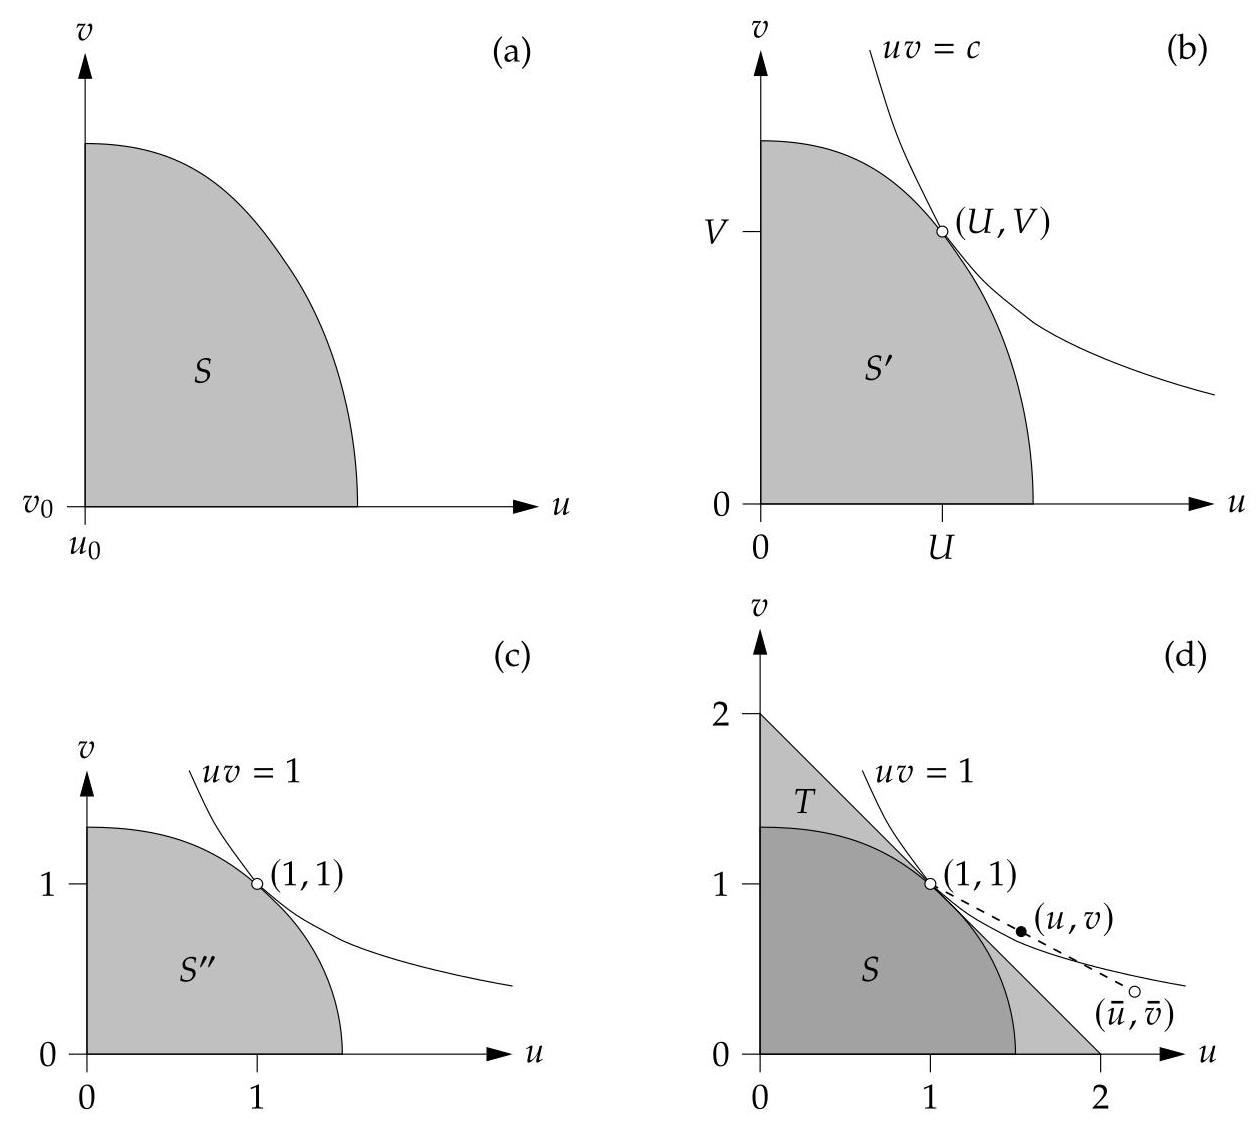
\includegraphics[width=0.9\textwidth]{translation/images/ch11-fig03.jpg}
\caption{展示了定理~\ref{theo:11.3}的证明步骤。(d)中的虚线表明，位于三角形 \(\left( {\bar{u},\bar{v}}\right)\) (深灰色和浅灰色)外部的点 \(T\) ，不可能属于 \(S\) (深灰色)，这表明 \(S \subseteq  T\)。}
\label{fig:11.3}
\end{figure}

为了正式证明这一点，考虑 \(\left( {U,V}\right)  = \left( {1,1}\right)\) 和 \(\left( {\bar{u},\bar{v}}\right)\) 的凸组合$(u,v)$的纳什积:
\begin{equation}
\label{eq:11.1}
\begin{aligned}
uv &= [(1 - \varepsilon)U + \varepsilon\bar{u}][(1 - \varepsilon)V + \varepsilon\bar{v}] \\
   &= [U + \varepsilon(\bar{u} - U)][V + \varepsilon(\bar{v} - V)] \\
   &= UV + \varepsilon\left[\bar{u} + \bar{v} - (U + V)
      + \varepsilon(\bar{u} - U)(\bar{v} - V)\right].
\end{aligned}
\end{equation}

现在，已知\(\bar{u} + \bar{v} > 2\)，且\(U + V = 2\)，因此 \(\bar{u} + \bar{v} - \left( {U + V}\right)\) 为正。即使 \(\left( {\bar{u} - U}\right) \left( {\bar{v} - V}\right)\) 是任意负数，只要选取足够小的正数\(\varepsilon  > 0\)，\(\varepsilon \left( {\bar{u} - U}\right) \left( {\bar{v} - V}\right)\) 的绝对值也可以小于 \(\bar{u} + \bar{v} - \left( {U + V}\right)\)。因此，取足够小的正 \(\varepsilon\)，可得 \({uv} > 1 = {UV}\)，这表明 \({UV}\) 不是 \(S\) 中的最大纳什积，这与我们对$(U,V)$的构造相矛盾。由此证得\(S \subseteq  T\)成立，进而可得前文的结论 \(N\left( S\right)  = N\left( T\right)\)。

为了证明点 \(\left( {U,V}\right)  = \left( {1,1}\right)\)是唯一的，我们依旧借助双曲线，采用和前文相同的论证思路。具体来说，假设 \(\left( {u,\frac{1}{u}}\right)\) 是双曲线 \(S\) 上的另一点，且 \(u \neq  1\)。由于 \(S\) 是凸集，连接$(1,1)$和 \(\left( {u,\frac{1}{u}}\right)\) 的线段也在 \(S\) 中，且该线段上所有内点的纳什积都更大。例如，中点 \(\frac{1}{2} \cdot  \left( {1,1}\right)  + \frac{1}{2} \cdot  \left( {u,\frac{1}{u}}\right)\) 的纳什积为 \(\left( {1 + u + \frac{1}{u} + u\frac{1}{u}}\right) /4\)，当且仅当 \(u + \frac{1}{u} > 2\) 时，该纳什积大于1，而\({\left( u - 1\right) }^{2} > 0\) 等价于 \({\left( u - 1\right) }^{2} > 0\)，又因为 \(u \neq  1\)故该不等式成立。因此，再次结合 \(S\) 是凸集这一条件可以推出，\(S\) 中的纳什积存在唯一的最大值。
\end{proof}

我们假设讨价还价集合 \(S\) 存在一个点 (u, v)，满足 \(u > {u}_{0}\) 和 \(v > {v}_{0}\)，该假设的意义如下：若不满足此假设，对于任意 \(\left( {u,v}\right)  \in  S\)，玩家 I 的所有效用 \(u\) 或玩家 II 的所有效用 \(v\) (或两者)分别满足 \(u = {u}_{0}\) 或 \(v = {v}_{0}\)。那么对于 \(\left( {u,v}\right)  \in  S\)，纳什积 \(\left( {u - {u}_{0}}\right) \left( {v - {v}_{0}}\right)\) 总是为零，所以除非 \(S\) 只是单元素集 \(\left\{  \left( {{u}_{0},{v}_{0}}\right) \right\}\)，否则它没有唯一的最大值。那么议价集 \(S\) 是一个单元素集或一条线段 \(\left\{  {u}_{0}\right\}   \times  \left\lbrack  {{v}_{0},V}\right\rbrack\) 或 \(\left\lbrack  {{u}_{0},U}\right\rbrack   \times  \left\{  {v}_{0}\right\}\)。在这种相当简单的情况下，帕累托前沿仅由一个单点 $(U,V)$ 组成，该点即为唯一的纳什解 \(N\left( S\right)\)。

\begin{tcolorbox}
\(\Rightarrow\) 若议价集如前文所述为一条线段，为何其帕累托前沿仅为单个点？若该线段不与任意一条坐标轴平行，该结论是否仍成立？
\end{tcolorbox}

可以相对容易地证明，定理~\ref{theo:11.3}中描述的纳什积最大化给出了一个满足定义~\ref{def:11.1}和~\ref{def:11.2}中公理的解 $(U,V)$。

\begin{tcolorbox}
\(\Rightarrow\) 练习~\ref{exer:11.1} 要求你针对公理(f)验证该结论。
\end{tcolorbox}

下面我们说明如何求解图~\ref{fig:11.1}中讨价还价集 \(S\) 的讨价还价解$(U,V)$。威胁点 \(\left( {{u}_{0},{v}_{0}}\right)\) 为$(1,1)$。帕累托前沿由两条线段组成:第一条线段连接$(1,3.5)$和$(2,3)$，第二条线段连接$(2,3)$和$(4,1)$，其中后者是从$(2,3)$延伸到$(5,0)$的更长线段的一部分（第一条线段也是连接$(4,0)$和$(2,3)$的更长线段的一部分，不过该信息后文用不到）。对于帕累托前沿上任意一点$(u,v)$，其纳什积 \(\left( {u - {u}_{0}}\right) \left( {v - {v}_{0}}\right)\) 是威胁点 \(\left( {{u}_{0},{v}_{0}}\right)\) 和点 \((u,v)\)之间矩形的面积大小。本例从图像能直观看出，第二段线段能构造出面积更大的矩形。第二段线段上任意一点可参数化为 \(\left( {1 - p}\right) \left( {2,3}\right)  + p\left( {5,0}\right)\)，其中 \(0 \leq  p \leq  1\) ，即 \(\left( {2 + {3p},3 - {3p}}\right)\)。结合 \(\left( {{u}_{0},{v}_{0}}\right)  = \left( {1,1}\right)\)，代入纳什积公式为\(\left( {1 + {3p}}\right) \left( {2 - {3p}}\right)\) 或 \(2 + {3p} - 9{p}^{2}\)。该表达式在 \(p\) 上的唯一最大值在 \(p = \frac{1}{6}\) 时取得，因为这是其导数 \(3 - {18p}\) 的零点，且二阶导数为负，所以这是一个极大值。因此，点$(U,V)$为$(2.5,2.5)$。一般来说，若极值解落在区间 \(p < 0\) 或 \(p > 1\) ，则纳什积最大值会取在线段端点\(p = 0\) 或 \(p = 1\)处。此时需要考察相邻线段，纳什积最大值有可能出现在两段线段衔接的拐点处。 借助该\(p\)值，纳什讨价还价解可以表示为双矩阵博弈中各组收益对的凸组合，具体通过一个抽签机制实现，以概率 \(1 - p = \frac{5}{6}\) 选择收益为$(2,3)$的策略组合$(T,l)$，以概率 \(p = \frac{1}{6}\) 选择收益为$(5,0)$的策略组合$(B,r)$。双方玩家事先已同意接受这个抽签机制的结果。尽管以概率 \(\frac{1}{6}\) 出现的收益对$(5,0)$会使玩家II的收益为零，这比她在威胁点获得的 \({v}_{0} = 1\) 要少；然而，她从抽签机制中获得的期望效用2.5高于 \({v}_{0}\)。


\section{\texorpdfstring{{\color{red}纳什}讨价还价解的几何性质}{纳什讨价还价解的几何性质}}\label{sec11.5}

在本节中，我们给出讨价还价解的几何特征。这一特征有助于快速找到讨价还价解，并且在第~\ref{sec11.11}~节中会用到。我们首先陈述一个简单的引理：

\begin{lemma}\label{lem:11.4}
考虑一个顶点为 \(\left( {0,0}\right),\left( {a,0}\right) ,\left( {0,b}\right)\) 且满足 \(a,b > 0\) 的三角形 \(T\)。那么包含在 \(T\) 中，顶点为 \(\left( {0,0}\right),\left( {U,0}\right) ,\left( {U,V}\right)\) 和$(0,V)$的最大面积矩形由 \(U = a/2\) 和 \(V = b/2\) 确定。此外，如果 \(S \subseteq  T\) 且 \(\left( {U,V}\right)  \in  S\)，那么$(U,V)$也是 \(S\) 中使乘积 \({UV}\) 最大的点。
\end{lemma}

\begin{figure}[htbp]
\centering
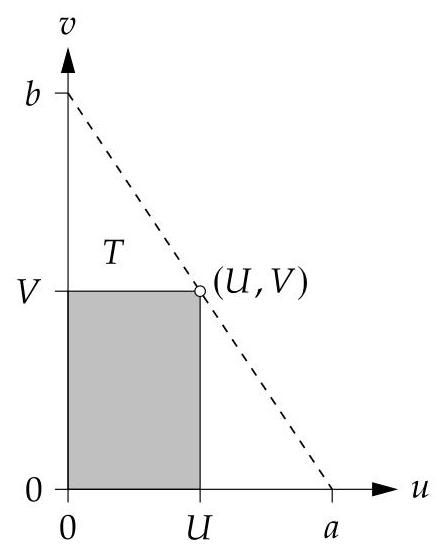
\includegraphics[width=0.3\textwidth]{translation/images/ch11-fig04.jpg}
\caption{是引理~\ref{lem:11.4}的图示。乘积 \({UV}\) 是内接于三角形 \(T\) 的灰色矩形的面积，当 \(U = a/2\) 和 \(V = b/2\) 时该面积最大。}
\label{fig:11.4}
\end{figure}

\begin{proof}乘积 \({UV}\) 是如图~\ref{fig:11.4}所示内接于 \(T\) 的矩形的面积。对于 \(\left( {u,v}\right)  \in  T\)， \({uv}\) 的最大值显然在$(u,v)$位于连接\textcolor{red}{$(0,b)$} 和$(a,0)$的直线上时取得，该直线在图~\ref{fig:11.4}中用虚线表示，该直线方程为 \(v = b - \frac{b}{a}u\)。构造函数 \(u \mapsto  u \cdot  \left( {b - \frac{b}{a}u}\right)\)，对$u$求一阶导数为 \(b - 2\frac{b}{a}u\)，令一阶导数等于 0，解得极值点\(u = a/2\)，又因为其二阶导数小于 0，该极值点为函数极大值点。综上可证，当 \(U = a/2\) 和 \(V = b/2\) 时， \({UV}\) 取得最大值。
\end{proof}

如果 \(S \subseteq  T\)，那么对于 \(\left( {u,v}\right)  \in  S\)， \({uv}\) 的最大值显然至多是对于 \(\left( {u,v}\right)  \in  T\) 时 \({uv}\) 的最大值，因此如果 \(\left( {U,V}\right)  \in  S\)，则在 \(\left( {u,v}\right)  = \left( {U,V}\right)\) 时取得。

以下命题给出了一个从几何角度寻找讨价还价解的有用条件。根据公理(c)，假设讨价还价集是凸集，威胁点为$(0,0)$，并且其帕累托前沿的形式为 \(\left( {u,f\left( u\right) }\right)\)，其中 \(f\) 是一个递减函数，为明确起见，令 \(0 \leq  u \leq  1\)，当然\(u\) 的区间右端点也可取其他数值。

\begin{proposition}\label{prop:11.5}假设威胁点为$(0,0)$的讨价还价集 \(S\) 的帕累托前沿由 \(\{ \left( {u,f\left( u\right) }\right)  \mid  0 \leq  u \leq  1\}\) 给出，其中 \(f\) 是一个递减且连续的函数，满足 \(f\left( 0\right)  > 0\) 和 \(f\left( 1\right)  = 0\)。那么讨价还价解$(U,V)$是讨价还价集有一条斜率为 \(- f\left( U\right) /U\) 的切线的唯一一点 \(\left( {U,f\left( U\right) }\right)\)。如果 \(f\) 可微，那么该斜率是 \(f\) 在 \(U\) 处的导数 \({f}^{\prime }\left( U\right)\)，即 \({f}^{\prime }\left( U\right)  =  - f\left( U\right) /U\)。
\end{proposition}

\begin{figure}[htbp]
\centering
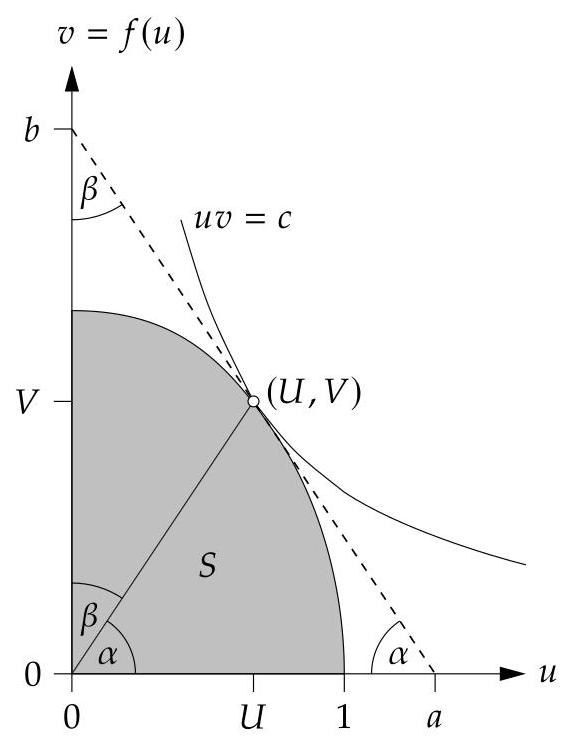
\includegraphics[width=0.4\textwidth]{translation/images/ch11-fig05.jpg}
\caption{命题~\ref{prop:11.5}及其证明的图示。虚线是双曲线 \(\{ \left( {u,v}\right)  \mid  {uv} = c = {UV}\}\) 在点 $(U,V)$ 处的切线，该切线也是讨价还价集 \(S\) 在点 $(U,V)$ 处的切线。此切线的端点 $(a,0)$ 和 $(0,b)$ 满足 \(a = {2U}\) 和 \(b = {2V}\)，夹角分别为 \(\alpha\) 和 \(\beta\)，如图所示。}
\label{fig:11.5}
\end{figure}

\begin{proof}
设 $(U,V)$ 是讨价还价集 \(S\) 的讨价还价解。它位于帕累托前沿上，因此 \(V = f\left( U\right)\)。设 \(c = {UV}\) 并考虑双曲线 \(\{ \left( {u,v}\right)  \mid  {uv} = c\}\)，根据定理~\ref{theo:11.3}，该双曲线与 \(S\) 仅在点 (U, V) 处相交。因为 (U, V) 使纳什积最大化，所以 \(c\) 是 \(c = {uv}\) 在 \(\left( {u,v}\right)  \in  S\) 上所能取到的最大值。函数 \(u \mapsto  c/u\) 可导，其导数为 \(- c/{u}^{2}\)，当 \(u = U\) 时，该导数等于 \(- V/U\)。考虑过点 $(U,V)$ 且斜率为 \(- V/U\) 的直线，此直线是双曲线在点 $(U,V)$ 处的切线，如图~\ref{fig:11.5}中的虚线所示。该直线与 \(u\) 轴相交于点 \(\left( {a,0}\right)  = \left( {{2U},0}\right)\)，与 \(v\) 轴相交于点 \(\left( {0,b}\right)  = \left( {0,{2V}}\right)\)，并定义了一个顶点为 \(\left( {0,0}\right),\left( {a,0}\right)\) 和 $(0,b)$ 的三角形 \(T\) 。图~\ref{fig:11.5}对应于图~\ref{fig:11.3}(b)，如果我们通过将 \(u\) 替换为 \(u/U\) 以及将 \(v\) 替换为 \(v/V\) 来重新缩放坐标轴，那么我们将得到图~\ref{fig:11.3}(d)，其中 \(T\) 是顶点为 \(\left( {0,0}\right),\left( {2,0}\right)\) 和 \(\left(0,2\right)\) 的三角形。借助 \eqref{eq:11.1} 我们证明了 \(S \subseteq  T\)，其中未使用假设 \(\left( {U,V}\right)  = \left( {1,1}\right)\)，因此这也适用于图~\ref{fig:11.5}，无需重新缩放坐标轴。据此，正如前文结论，虚线同样是集合\(S\)的一条切线。

如果函数 \(f\) 不可微，那么在某一点处集合 \(S\) 可能存在多条切线。在这种情况下，仍需证明按上述方式构造出的$(U,V)$ 是唯一的。假设 \(S\) 的一条切线与 \(S\) 相切于点 $(U,V)$，且斜率为负，等于 \(- V/U\)，并如图~\ref{fig:11.5}所示，切线与 \(u\) 轴相交于 $(a,0)$，与 \(v\) 轴相交于 $(0,b)$，（现在我们忽略双曲线）。切线的斜率 \(- V/U\) 意味着 \(a = {2U}\) 和 \(b = {2V}\)。作为集合 \(S\) 的切线意味着 \(S\) 是顶点为 \(\left( {0,0}\right),\left( {a,0}\right)\) 和 $(0,b)$ 的三角形 \(T\) 的子集。根据引理~\ref{lem:11.4}， \({UV}\) 是 \({uv}\) 在 \(\left( {u,v}\right)  \in  S\) 条件下的最大值。由此即可说明 $(U,V)$ 是唯一的。

如果函数 \(f\) 可微，那么集合 \(S\) 在每一点处的切线都是唯一的，我们可以直接进行如下论证。讨价还价解在帕累托前沿上使纳什积 \(u \cdot  f\left( u\right)\) 最大化。这要求关于 \(u\) 的导数为零，即 \(f\left( u\right)  + u \cdot  {f}^{\prime }\left( u\right)  = 0\) 或 \({f}^{\prime }\left( u\right)  =  - f\left( u\right) /u\)，因此 \(U\) 必须满足这个方程，证毕。
\end{proof}

在图~\ref{fig:11.5} 中，点 $(U,V)$ 是直角三角形长边的中点，该直角三角形的顶点为 $(0,0)$，$(a,0)$ 和 $(0,b)$。从 $(0,0)$ 到 $(U,V)$ 的直线将该三角形分成两个等腰三角形。第一个三角形的顶点为 $(U,V)$，在其顶点 $(0,0)$ 和 $(a,0)$ 处有相等（镜像对称）的角 \(\alpha\)。这些角对应于连接这些顶点与 $(U,V)$ 的两条直线的斜率 \(V/U\) 和 \(- V/U\)，二者斜率绝对值相等、符号相反。第二个三角形的顶点为 $(U,V)$，在其顶点 $(0,0)$ 和 $(0,b)$ 处有相等（镜像对称）的角 \(\beta\)。

图~\ref{fig:11.6} 展示了讨价还价集 \(S\)，其帕累托前沿由线段给出，当 \(S\) 从如图~\ref{fig:11.1} 所示的双矩阵博弈中推导得出时就会出现这种情况（将威胁点移至$(0,0)$，就得到了图~\ref{fig:11.6}(b) 中所示的集合）。然后，借助引理~\ref{lem:11.4} 可以轻松找到纳什讨价还价解：找到与端点为 $(a,0)$ 和 $(0,b)$ 的讨价还价集 \(S\) 相切的切线，使得该切线的中点 $(U,V)$ 属于 \(S\) （命题~\ref{prop:11.5} 保证了这条切线存在）。因为 \(S\) 的边界由线段组成，所以线段内部点处的切线与该线段具有相同的斜率，因此只需检查有限多个斜率。在图~\ref{fig:11.6}(a) 中，对应的切线中点 $(U,V)$ 落在中间那条边界线段上。

仅由两段线段构成帕累托前沿的情形求解尤为简便。在图~\ref{fig:11.6}(b) 中，右侧的线段包含相应切线的中点 $(U,V)$。该切线和线段具有相同的右端点 $(a,0)$，这意味着 \(U = \frac{a}{2}\)。类似地，在图~\ref{fig:11.6}(c) 中，顶部的线段包含相应切线的中点 $(U,V)$。该切线和线段具有相同的左端点 $(0,b)$，这意味着 \(V = \frac{b}{2}\)。在图~\ref{fig:11.6}(d) 中，没有一条线段能定义出其中点属于 \(S\) 的切线，因为右侧的线段太陡，而顶部的线段太平缓。那么讨价还价集 \(S\) 的顶点 $(U,V)$ 就是纳什讨价还价解；这可以通过考虑过该顶点且斜率为 \(- V/U\) 的虚线来验证，该斜率是从 $(0,0)$ 到 $(U,V)$ 的直线斜率 \(V/U\) 的负值，与 \(u\) 轴的夹角为 \(\alpha\)。这条线应该是 \(S\) 的切线，本图情形正是如此。

\begin{figure}[htbp]
\centering
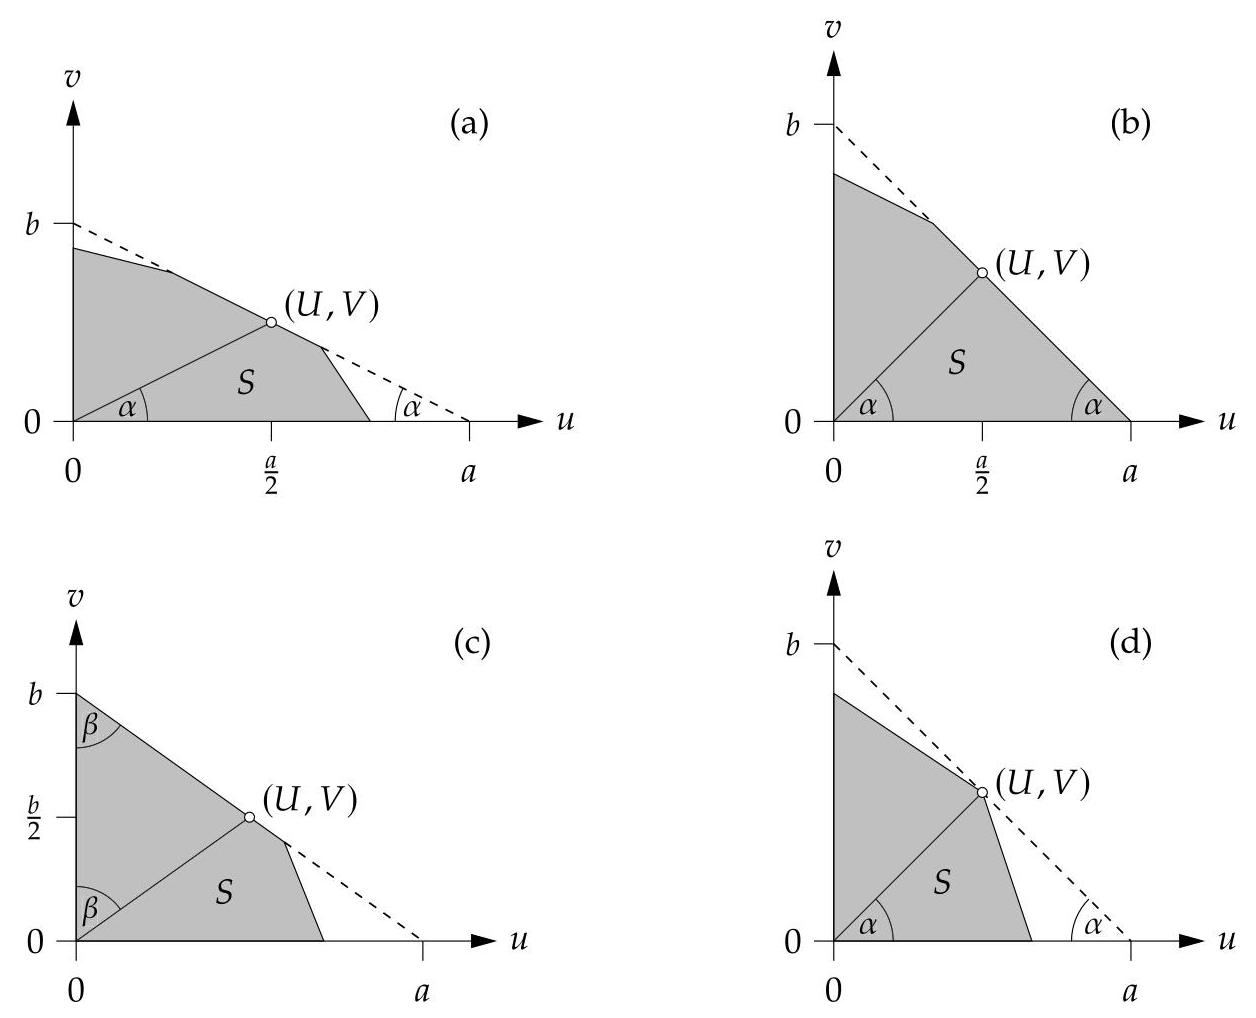
\includegraphics[width=0.9\textwidth]{translation/images/ch11-fig06.jpg}
\caption{展示了具有分段线性帕累托前沿的各种讨价还价集 \(S\) 。根据命题~\ref{prop:11.5}，纳什讨价还价解$(U,V)$ 是与 \(S\) 相切的切线(虚线)落在第一象限内截得线段的中点，线段的端点为 $(a,0)$ 和 $(0,b)$。在 (d) 中，点 $(U,V)$ 是 \(S\) 的一个顶点，过该点有许多与 \(S\) 相切的切线。其中一条切线与 \(u\) 轴的夹角 \(\alpha\) 与从 $(0,0)$ 向上到 $(U,V)$ 的直线的夹角相同。}
\label{fig:11.6}
\end{figure}




\section{分蛋糕问题}\label{sec11.6}

在本章的其余部分，我们考虑一个讨价还价的情形，其中参与者I和参与者II必须达成协议来分割一个蛋糕，参与者I分得 \(x\)，参与者II分得\(y\)。待分割的总量被规范化为一个单位，因此该模型称为单位蛋糕模型。所有可行的分配方案 $(x,y)$ 必须满足 \(x \geq  0,y \geq  0\) 以及 \(x + y \leq  1\)。如果两个参与者无法达成一致，则双方收益均为 0，由此确定威胁点 $(0,0)$。满足 \(x + y < 1\) 的分配方案 $(x,y)$ 不是帕累托最优的，但为了得到一个凸集，我们仍把这类分配纳入可行集。

\begin{figure}[htbp]
\centering
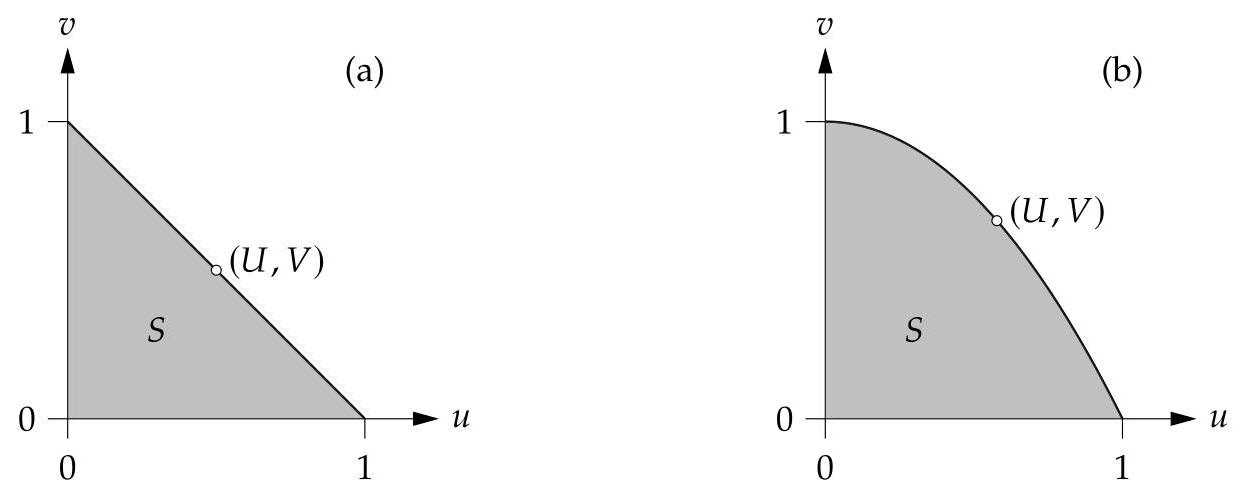
\includegraphics[width=0.9\textwidth]{translation/images/ch11-fig07.jpg}
\caption{关于单位蛋糕的讨价还价，讨价还价集 \(S\) 如 \eqref{eq:11.2} 中所定义。在 (a) 中，效用函数为 \(u\left( x\right)  = x\) 和 \(v\left( y\right)  = y\)，讨价还价解为 \(\left( {U,V}\right)  = \left( {\frac{1}{2},\frac{1}{2}}\right)\)。在 (b) 中，它们是 \(u\left( x\right)  = \sqrt{x}\) 和 \(v\left( y\right)  = y\)，讨价还价解为 \(\left( {U,V}\right)  = \left( {1/\sqrt{3},\frac{2}{3}}\right)  \approx  \left( {{0.577},{0.667}}\right)\)。}
\label{fig:11.7}
\end{figure}

如果参与者I获得效用 \(x\)，参与者II获得效用 \(y\)，那么讨价还价集就是所有满足 \(x \geq  0,y \geq  0\) 和 \(x + y \leq  1\) 的数对 $(x,y)$ 所构成的三角形，如图~\ref{fig:11.7}(a) 所示。如果 \(x + y = 1\)，则分割方案 $(x,y)$ 是帕累托最优的，因此帕累托前沿由分割方案 $(x,1-x)$ 给出，在图中用粗线表示。因为威胁点是 $(0,0)$，所以纳什积为 \(x\left( {1 - x}\right)\)，当 \(x = \frac{1}{2}\) 时该纳什积达到最大值。纳什讨价还价解 \(\left( {U,V}\right)  = \left( {\frac{1}{2},\frac{1}{2}}\right)\) 也可由定义~\ref{def:11.2}(g) 中的对称性公理得出。

我们考虑更一般的蛋糕分配问题，其中参与者的效用函数 \(u\) 和 \(v\) 不是恒等函数。我们假设参与者 \(\mathrm{I}\) 的效用函数为 \(u : \left\lbrack  {0,1}\right\rbrack   \rightarrow  \left\lbrack  {0,1}\right\rbrack\)，参与者 \(\mathrm{{II}}\) 的效用函数为 \(v : \left\lbrack  {0,1}\right\rbrack   \rightarrow  \left\lbrack  {0,1}\right\rbrack\)，并且这些效用函数经过了规范化处理，使得 \(u\left( 0\right)  = v\left( 0\right)  = 0\)，\(u\left( 1\right)  = v\left( 1\right)  = 1\)。进一步假设这些效用函数是递增的、凹的（见式~\eqref{eq:5.46}和图~\ref{fig:5.5}）且连续的（可以证明，除了函数定义域的端点外，凹性意味着连续性）。两个参与者所得到的效用对的讨价还价集由下面的式子决定：
\begin{equation}
\label{eq:11.2}
S = \{ \left( {u\left( x\right) ,v\left( y\right) }\right)  \mid  x \geq  0,y \geq  0,x + y \leq  1\}.
\end{equation}

以下命题说明了 \(S\) 满足定义~\ref{def:11.1}中的公理:

\begin{proposition}\label{prop:11.6}
设 \(u,v : \left\lbrack  {0,1}\right\rbrack   \rightarrow  \mathbb{R}\) 分别为参与者 \(I\) 和 \({II}\) 的递增、凹且连续的效用函数，其中 \(u\left( 0\right)  = v\left( 0\right)  = 0\) 且 \(u\left( 1\right)  = v\left( 1\right)  = 1\)。那么，由\eqref{eq:11.2}定义的议价集 \(S\) 的威胁点为$(0,0)$，并且\(S\)是紧致且凸的。此外，\(S\) 是向下闭合的，即
\begin{equation}
\label{eq:11.3}
\left( {\bar{u},\bar{v}}\right)  \in  S,\;0 \leq  {u}^{\prime } \leq  \bar{u},\;0 \leq  {v}^{\prime } \leq  \bar{v}\; \Rightarrow  \;\left( {{u}^{\prime },{v}^{\prime }}\right)  \in  S.
\end{equation}
\end{proposition}

\begin{proof}
我们首先证明\eqref{eq:11.3}。设 \(0 \leq  {u}^{\prime } \leq  \bar{u}\) 且 \(0 \leq  {v}^{\prime } \leq  \bar{v}\)，且 \(\left( {\bar{u},\bar{v}}\right)  \in  S\)，即对于某些满足 \(\bar{x} + \bar{y} \leq  1\) 的 \(\bar{x} \geq  0\) 和 \(\bar{y} \geq  0\)，有 \(\bar{u} = u\left(\bar{x}\right)\) 且 \(\bar{v} = \textcolor{red}{v}\left(\bar{y}\right)\)。因为 \(u\left( 0\right)  = 0 \leq  {u}^{\prime } \leq  u\left( \bar{x}\right)\) 且 \(u\) 是连续的，根据介值定理，对于某些 \({x}^{\prime } \in  \left\lbrack  {0,\bar{x}}\right\rbrack\) 有 \(u\left( {x}^{\prime }\right)  = {u}^{\prime }\)，类似地，对于某些 \({y}^{\prime } \in  \left\lbrack  {0,\bar{y}}\right\rbrack\) 有 \(v\left( {y}^{\prime }\right)  = \textcolor{red}{v}^{\prime }\)，这意味着 \({x}^{\prime } + {y}^{\prime } \leq  \bar{x} + \bar{y} \leq  1\)，从而 \(\left( {{u}^{\prime },{v}^{\prime }}\right)  \in  S\)，这就证明了\eqref{eq:11.3}。

集合 \(S\) 是紧集在连续函数 \(\left( {x,y}\right)  \mapsto\)  \(\left( {u\left( x\right) ,v\left( y\right) }\right)\) 下的映像，因此它也是紧集。为了证明 \(S\) 是凸集，任取\(S\) 内两点做凸组合 \(\left( {{u}^{\prime },{v}^{\prime }}\right)  = \left( {1 - \lambda }\right) \left( {u\left( x\right),v\left( y\right) }\right)  + \lambda \left( {u\left( \widetilde{x}\right),v\left( \widetilde{y}\right) }\right)\) ，其中 \(\lambda  \in  \left\lbrack  {0,1}\right\rbrack\)。因为 \(u\) 和 \(v\) 是凹函数，有 \({u}^{\prime } \leq  u\left( {\left( {1 - \lambda }\right) x + \lambda \widetilde{x}}\right)  = \bar{u}\) 且 \({v}^{\prime } \leq  v\left( {\left( {1 - \lambda }\right) y + \lambda \widetilde{y}}\right)  = \bar{v}\)，显然 \(\left( {\bar{u},\bar{v}}\right)  \in  S\)。此外， \({u}^{\prime } \geq  0\) 且 \({v}^{\prime } \geq  0\)。因此，\eqref{eq:11.3} 式意味着 \(\left( {{u}^{\prime },{v}^{\prime }}\right)  \in  S\)，这表明 \(S\) 是凸集。
\end{proof}

对于效用函数 \(u\left( x\right)  = \sqrt{x}\) 和 \(v\left( y\right)  = y\)，集合 \(S\) 如图~\ref{fig:11.7}(b) 所示。帕累托前沿由满足 \(0 \leq  x \leq  1\) 的点 \(\left( {u\left( x\right),v\left( {1 - x}\right) }\right)\) 给出。因为 \(u = \sqrt{x}\) 和 \(v = 1 - x = 1 - {u}^{2}\)，因此这些点可以写为 \(\left( {u,1 - {u}^{2}}\right)\)，于是 \(v\) 可直接表示为关于 \(u\) 的函数 \(1 - {u}^{2}\)。一般来说，可以把改变参数 \(x\) ，看作遍历帕累托前沿上的点 \(\left( {u\left( x\right),v\left( {1 - x}\right) }\right)\)，从 \(x = 0\) 时前沿的上端点 (0,1)，到 \(x = 1\) 时前沿的右端点 (1,0)。

纳什讨价还价解$(U,V)$ 是通过在帕累托前沿上最大化纳什积 \(u\left( x\right) v\left( {1 - x}\right)\) 得到的。在图~\ref{fig:11.7}(b) 中，纳什积为 \(\sqrt{x}\left( {1 - x}\right)\) 或 \({x}^{1/2} - {x}^{3/2}\)，其导数为 \(\frac{1}{2}{x}^{-1/2} - \frac{3}{2}{x}^{1/2}\) 或 \(\frac{1}{2}{x}^{-1/2}\left( {1 - {3x}}\right)\)，当 \(x = \frac{1}{3}\) 时导数为零，且二阶导数为负，因此该点取到最大值。因此，蛋糕的\(\frac{1}{3}\)被分给参与者 I，\(\frac{2}{3}\) 被分给参与者 II。相应的效用对 $(U,V)$ 为 \(\left( {1/\sqrt{3},\frac{2}{3}}\right)\)，约为 $(0.577,0.667)$。针对其他效用函数的同类计算，参见练习~\ref{exer:11.4}。




\section{最后通牒博弈}\label{sec11.7}

假设如前一节所述，两名参与者必须分割一单位的蛋糕。接下来，我们将构建适用于这种情况的“交替出价”讨价还价博弈。这是一个非合作博弈，用于模拟参与者在讨价还价情境中可能的互动方式。对于这一非合作博弈，其最完整的“平稳策略”版本的解（见第~\ref{sec11.10}~节），将逼近纳什讨价还价解。该模型通过另一种不同的角度来证明纳什解的合理性，这种方法不是公理化的，而是使用了博弈树中的子博弈完美均衡概念。

该模型规定，蛋糕根据其中一名参与者的提议进行分配。假设参与者I提议将蛋糕分为两部分：参与者I得到 \(x\)，参与者II得到 \(1 - x\)，这样参与者分别获得效用 \(u\left( x\right)\) 和 \(v\left( {1 - x}\right)\)。参与者I提出的数量 \(x\) 也被称为他的{\textcolor{blue}要求}，因为这是他在提议的分配方案中所获得的蛋糕份额。

\begin{figure}[htbp]
\centering
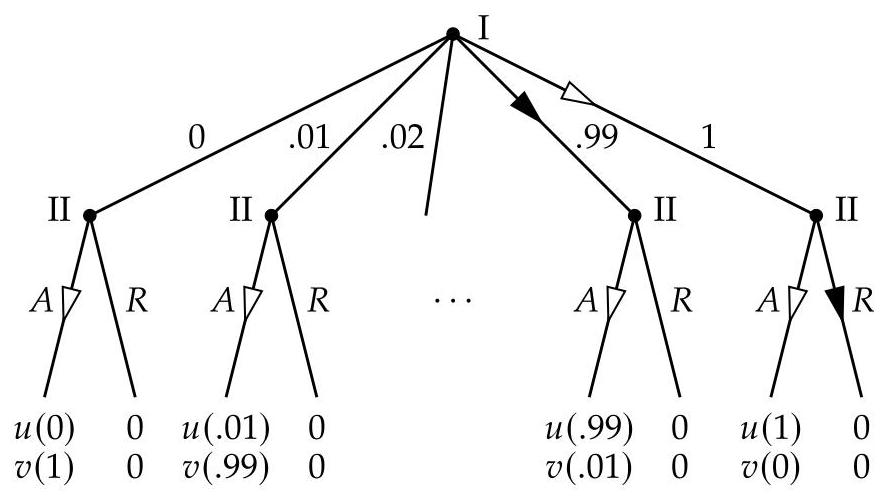
\includegraphics[width=0.6\textwidth]{translation/images/ch11-fig08.jpg}
\caption{展示了最后通牒博弈的离散版本。黑色与白色箭头分别表示两个子博弈完美均衡，两个均衡几乎完全相同，唯一区别在于：参与者II对参与者I要求全部蛋糕$x=1$时如何回应，以及与之对应的参与人I的最优反应为$x=0.99$或$x=1$。}
\label{fig:11.8}
\end{figure}

在最基本的形式下，这个模型被称为最后通牒博弈，在这个博弈中，参与者II可以接受或拒绝该分配方案。如果参与者II接受，收益组合为 \(\left( {u\left( x\right) ,v\left( {1 - x}\right) }\right)\)；如果她拒绝，收益组合为(0,0)，在这种情况下，两名参与者都得不到任何东西。图~\ref{fig:11.8}展示了这个博弈的离散版本，其中可能的需求 \(x\) 是0.01的倍数。因此，参与者I有101种可能的行动，即 \(x \in  \left\{  {\left. \frac{i}{100}\right| \;i = 0,1,\ldots,{100}}\right\}\)，并且对于参与者I提出的每个 \(x\)，参与者II可以选择 \(A\)（接受）或 \(R\) （拒绝）。因此，参与者II有 \({2}^{101}\) 种纯策略，这些策略由每个可能的 \(x\) 对应的 \(A\) 和 \(R\) 的不同组合给出。

该博弈如图~\ref{fig:11.8}所示，我们要寻找该博弈的子博弈完美均衡，也就是说，因为该博弈具有完美信息，我们应用逆向归纳法。只要 \(1 - x > 0\)，参与者II的效用 \(v\left( {1 - x}\right)\) 就是正的，否则
\[
0 = v\left( {1 - x}\right)  = v\left( {x \cdot  0 + \left( {1 - x}\right)  \cdot  1}\right)  < 1 - x = x \cdot  v\left( 0\right)  + \left( {1 - x}\right)  \cdot  v\left( 1\right),
\]
这与 \(v\) 的凹性相矛盾（从图上也能看出）。因此，子博弈完美均衡条件意味着玩家 II 会接受玩家 I 提供的任何正数量 \(1 - x\)。这些通过逆向归纳法确定的选择在图~\ref{fig:11.8} 中用箭头表示，并且除了 \(x = 1\) （即玩家 I 要求获得整个蛋糕）的情况外，这些选择都是唯一的。在\(x = 1\)时，玩家 II 在接受和拒绝之间无差异，因为在这两种情况下她都得不到任何东西。因此，就纯策略而言， \({AA}\cdots {AA}\) 和 \({AA}\cdots {AR}\) 都是玩家 II 的子博弈完美均衡策略。这里，前 100 个 \(A\) 表示对每个 \(x = 0,{0.01},\ldots,{0.99}\) 的接受，最后一个 \(A\) 或 \(R\) 是当 \(x = 1\) 时的选择，分别在图~\ref{fig:11.8} 中用白色或黑色箭头表示。给定玩家 II 的这个策略，玩家 I 的最优反应是最大化他的收益，这通过玩家 I 对应的白色或黑色箭头来表示。如果玩家 II 接受要求 \(x = 1\)，那么玩家 I 会要求 \(x = 1\)，因此策略组合 \(\left( {1,{AA}\cdots {AA}}\right)\) 构成一个子博弈完美均衡；如果玩家 II 拒绝要求 \(x = 1\)，那么玩家 I 会要求 \(x = {0.99}\) （因为如果要求 \(x = 1\) 他将得不到任何东西），因此得到的子博弈完美均衡是 \(\left( {{0.99},{AA}\cdots {AR}}\right)\)。这两个策略组合是两个纯策略子博弈完美均衡。如果 \(u\left( {0.99}\right)  < 1\)，它们也是仅有的两个纯策略子博弈完美均衡；如果 \(u\left( {0.99}\right)  = 1\)，那么当玩家 II 采取接受所有要求的策略\({AA}\cdots {AA}\)时，要求 \(x = {0.99}\) 对玩家 I 来说也是一个最优反应。

本质上，在最后通牒博弈中，由于逆向归纳的假设，参与人 II 几乎无法获得任何收益。这一结论与此类现实议价场景中的人类行为并不相符，而这一点也已在最后通牒博弈的实验室实验中得到验证。这类实验的典型流程如下：玩家 I 在玩家 II 不知情的情况下声明他的要求 \(x\)，玩家 II 在玩家 I 不知情的情况下同时声明她自己的“保留要求” \(z\)；这两个玩家甚至可以从众多分别扮演玩家 I 和玩家 II 角色的受试者群体中匿名配对。只要 \(1 - x \geq  z\)，即给玩家 II 的提议至少和她的保留要求一样大，两个玩家就分别得到 \(x\) 和 \(1 - x\)，否则什么都得不到。（所以可能出现这样的情况，玩家 II 可以报一个很低的保留要求，比如 \(z = {0.01}\)，但仍然能得到 $0.4$，因为玩家 I 的要求是 \(x = {0.6}\)；这两者都可以被视为合理的选择，但它们不是相互的最优反应。）在这样的实验中，玩家 II 经常提出像 \(z = {0.4}\) 这样的正保留要求，玩家 I 提出像 \(x = {0.5}\) 这样谨慎的要求，这与子博弈完美均衡假设相矛盾。因此，对这些实验更好的描述可能是非子博弈完美的均衡，其中玩家 II“威胁”拒绝过低的提议 \(1 - x\)。尽管如此，我们仍采用子博弈完美均衡这一假设，原因有二：其一，该假设能让我们推导出明确的研究结论；其二，后续我们将通过设定 “拒绝提议后可提出反要求” 的规则，对模型进行优化与现实化改进。（练习~\ref{exer:11.3} 要求你找出离散最后通牒博弈的所有均衡。）

在离散型最后通牒博弈中，只要蛋糕可被划分为\(M + 1\)种可能的分配方案\((x,1 - x)\)（其中\(x = \frac{i}{M}\)，且\(i = 0,1,\ldots ,M - 1,M\)，如前文所述的\(M = 100\)的情形，上述两种子博弈完美均衡就必然存在。在她的 \({2}^{M + 1}\) 种纯策略中，玩家 II 在子博弈完美均衡中只能采用两种策略，即每当 \(x < 1\) 时总是选择 \(A\)，而面对 \(x = 1\)时选择 \(A\) 或 \(R\)。对应的玩家 \(\mathrm{I}\) 相应的要求是 \(x = 1\) 或 \(x = 1 - \frac{1}{M}\)。当离散化程度很高，即 \(M\) 趋近于无穷大时，这两种子博弈完美均衡几乎相同，玩家 I 要求得到全部（或几乎全部）蛋糕，而玩家 II 几乎一无所获。

\begin{figure}[htbp]
\centering
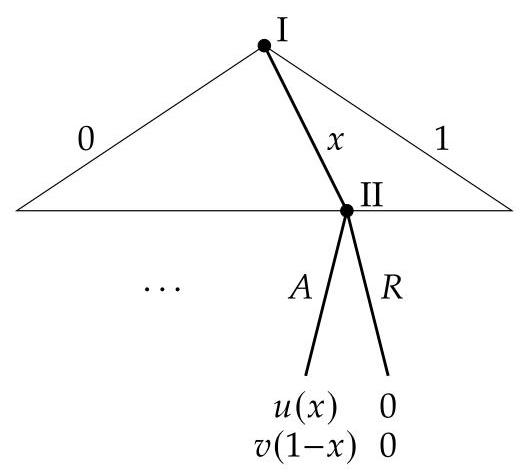
\includegraphics[width=0.4\textwidth]{translation/images/ch11-fig09.jpg}
\caption{连续最后通牒博弈。玩家 I 提出任何要求 \(x \in  \left\lbrack  {0,1}\right\rbrack\)，玩家 II 可以选择接受(A)或拒绝(R)。这里只展示了玩家 II 的一个决策。}
\label{fig:11.9}
\end{figure}

在连续最后通牒博弈中，玩家 \(\mathrm{I}\) 可能提出的要求 \(x\) 是区间 \(\left\lbrack  {0,1}\right\rbrack\) 内的任意数字，这为玩家 I 定义了无限种策略。玩家 II 的一种策略由一个函数 \(f : \left\lbrack  {0,1}\right\rbrack   \rightarrow  \{ A,R\}\) 给出，其中 \(f\left( x\right)  = A\) 表示玩家 II 接受要求 \(x\) ， \(f\left( x\right)  = R\) 表示玩家 II 拒绝该要求。（等价地，玩家 II 的一种策略是 \(\left\lbrack  {0,1}\right\rbrack\) 的任意一个子集，该子集恰好由她接受的那些要求 \(x\) 组成。）这个无限博弈如图~\ref{fig:11.9} 所示。无限多种选择 \(x\) 由三角形表示，其底边代表区间 \(\left\lbrack  {0,1}\right\rbrack\)。底边的每个点都对应玩家 II 的一个单独决策点，她可以在 \(A\) 和 \(R\) 之间做出选择。

我们要证明连续最后通牒博弈有唯一的子博弈完美均衡。这需要一个额外的假设，即玩家 \(\mathrm{I}\) 的效用函数 \(u\) 是严格递增的。如果满足下面引理中的 \({x}^{\prime } = 1\)，就满足该条件。

\begin{lemma}\label{lem:11.7}
设 \(u : \left\lbrack  {0,1}\right\rbrack   \rightarrow  \mathbb{R}\) 是一个递增、凹且连续的函数，满足 \(u\left( 0\right)  = 0\) 和 \(u\left( 1\right)  = 1\)。那么存在区间\(\left\lbrack  {0,{x}^{\prime }}\right\rbrack\)，使得\(u\) 在该区间上是严格递增的，并且对于所有的 \(x \in  \left\lbrack  {{x}^{\prime },1}\right\rbrack\) 有 \(u\left( x\right)  = 1\)。
\end{lemma}

\begin{proof}
集合$I = \{ x \in [0,1] \mid u(x) = 1 \}$非空（因为显然包含元素1），且因函数$u$的连续性可知该集合为闭集。设$x'$为集合$I$的最小元，则有$u(x') = u(1) = 1$。由于当$x' \leq x \leq 1$时，必有$1 = u(x') \leq u(x) \leq u(1) = 1$，故$I = [x',1]$。又因$u(0) = 0 < 1$，可得$x' > 0$。下证函数$u$在区间$[0,x']$上严格递增：假设该区间内存在两点$\bar{x}$和$\widehat{x}$满足$\bar{x} < \widehat{x}$，但$u(\bar{x}) = u(\widehat{x}) < u(x') = 1$。此时易知（结合图像可更直观理解），点$u(\widehat{x})$落在连接$u(\bar{x})$与$u(x')$的直线下方，而这与函数$u$的凹性相矛盾。
\end{proof}

如果引理~\ref{lem:11.7} 中的 \({x}^{\prime } < 1\) 成立，那么玩家 \(\mathrm{I}\) 仅获得 \({x}^{\prime }\) 就会完全满意，而 \({x}^{\prime }\) 小于整个蛋糕的份额。那么任何满足 \({x}^{\prime } \leq  x < 1\) 的要求 \(x\) 都会被玩家 II 接受，因为她能得到 \(v\left( {1 - x}\right)  > 0\)，并且 \(x\) 是玩家 I 在子博弈完美均衡中的一个可能策略。在这种情况下，我们无法得到唯一的子博弈完美均衡。因此，我们要求 \(u\) 严格递增，或者等价地，根据引理~\ref{lem:11.7}， \(u\left( x\right)  = 1\) 意味着 \(x = 1\)。因此，我们假设玩家 \(\mathrm{I}\) 的效用函数 \(u\)，以及类似地玩家 II 的效用函数 \(v\)，都是严格递增的。

以下命题表明，连续最后通牒博弈的唯一子博弈完美均衡是玩家 I 提出独占全部蛋糕的分配要求，即 \(x = 1\)，并且玩家 II 接受任何要求，包括在均衡路径上的要求 \(x = 1\)，因为在该均衡路径上她对接受和拒绝无差异。该均衡的推导逻辑并非简单将其视为离散型最后通牒博弈子博弈完美均衡的 “极限形式”，而是具有更严谨的深层内涵。

\begin{proposition}\label{prop:11.8}
设 \(u,v : \left\lbrack  {0,1}\right\rbrack   \rightarrow  \mathbb{R}\) 分别是玩家 \(I\) 和 \({II}\) 的严格递增、凹且连续的效用函数，且满足 \(u\left( 0\right)  = v\left( 0\right)  = 0\) 和 \(u\left( 1\right)  = v\left( 1\right)  = 1\)。那么连续最后通牒博弈有唯一的子博弈完美均衡：玩家 I 提出的分配要求为 \(x = 1\)，玩家 II 总是选择 \(A\)。
\end{proposition}

\begin{proof}
所描述的策略定义了一个子博弈完美均衡。为了证明其唯一性，首先观察到，只要 \(x < 1\)，玩家 II 就必须接受，因为此时她能获得正收益 \(v\left( {1 - x}\right)\)。假设存在一个子博弈完美均衡，其中玩家 I 的要求满足 \(x < 1\)。由于 \(u\) 是严格递增的，玩家 I 可以稍微提高索取额（仍少于 1，例如 \(\frac{x + 1}{2}\)），玩家 II 仍然会接受，此时玩家 I 能获得更多收益。因此， \(x = 1\) 是玩家 I 在子博弈完美均衡中的唯一策略。在均衡路径上，面对\(x = 1\)玩家 II 在选择 \(A\) 和 \(R\)之间无差异，甚至可以在二者之间随机选择。假设玩家 II以正概率 \(\varepsilon  > 0\) 选择 \(R\)，这使得玩家 I 的期望效用为 \(\left( {1 - \varepsilon }\right) u\left( 1\right)  + {\varepsilon u}\left( 0\right)\)，即 \(1 - \varepsilon\)。但这样一来，玩家 I 针对玩家 II 该策略的最优反应就不会是 \(x = 1\)。相反，玩家 I 可以提高自己的收益，例如要求 \(1 - \frac{\varepsilon }{2}\)，因为此时玩家 II 肯定会接受，玩家 I 能获得 \(u\left( {1 - \frac{\varepsilon }{2}}\right)  \geq  1 - \frac{\varepsilon }{2} > 1 - \varepsilon\)。但子博弈完美均衡中不允许索取额小于 1。因此，如果玩家 II \textcolor{red}{不是}以概率 1 接受要求 \(x=1\)，那么玩家 II 的这种反应并不能定义一个子博弈完美均衡。故上述子博弈完美均衡是唯一的。
\end{proof}

综上，在分配要求可连续选取的情形下，子博弈完美均衡中参与人的出价策略，会使另一方在接受与拒绝之间处于效用无差异状态，而后者仍会确定地选择接受。这一规律也将成为后续我们研究更复杂博弈中子博弈完美均衡的指导原则。




\section{两轮交替报价}\label{sec11.8}

接下来，我们扩展讨价还价模型：一旦一个玩家拒绝了另一个玩家的要求，她可以提出反要求，而另一个玩家又可以接受或拒绝该反要求。为了通过逆向归纳法找到这个博弈的子博弈完美均衡，这种交替出价必须在有限轮次后终止。最简单的情况是两轮讨价还价，本节将对此进行讨论。在第一轮中，玩家 I 提出要求 \(x\)，玩家 II 可以接受或拒绝。如果拒绝，她可以提出反要求 \(y\)，这代表她为自己争取的份额，因此蛋糕被分割为玩家 I 得到 \(1 - y\)，玩家 II 得到 \(y\)。如果玩家 I 接受该要求，他获得效用 \(u\left( {1 - y}\right)\)，玩家 II 获得效用 \(v\left( y\right)\)。如果玩家 \(\mathrm{I}\) 拒绝最终要求，两个玩家的收益都为零。

\begin{figure}[htbp]
\centering
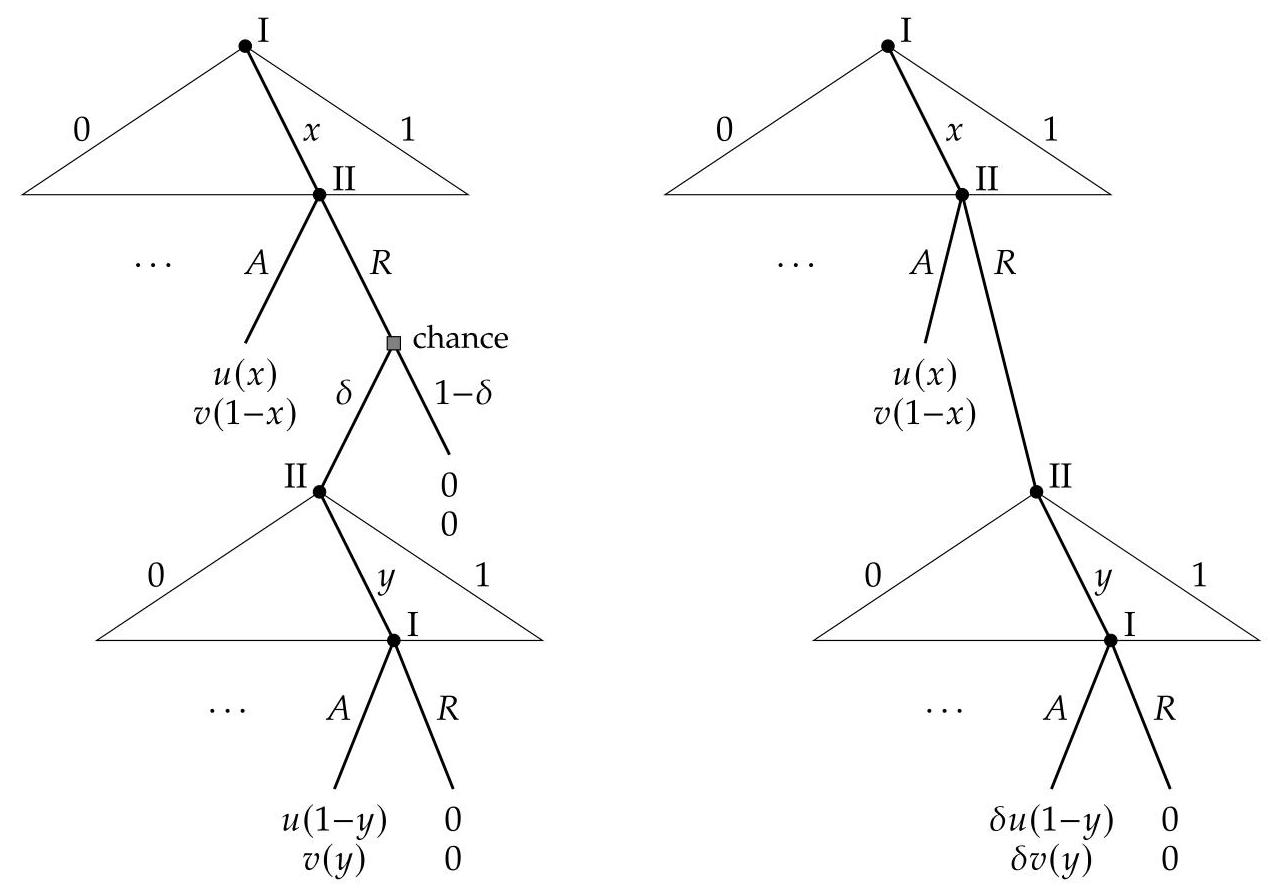
\includegraphics[width=1.0\textwidth]{translation/images/ch11-fig10.jpg}
\caption{两轮讨价还价，第一轮玩家 I 提出要求 \(x\)，第二轮玩家 II 提出反要求 \(y\)。左图:第二轮以概率 \(\delta\) 发生，否则以收益 $(0,0)$ 结束博弈。右图:简化的等价博弈，其中 \(\delta\) 作为贴现因子应用于第二轮的效用值。}
\label{fig:11.10}
\end{figure}

在这个博弈中，玩家 II 在最后一轮的要求是最终要求。因此，这个子博弈是玩家角色互换的最后通牒博弈，根据命题~\ref{prop:11.8}，玩家 II 可以要求整个蛋糕，因此，她在首轮中接受任何分配方案均无收益激励。出于这个原因，该模型设置了一个如图~\ref{fig:11.10} 所示的附加特征：当玩家 II 拒绝了首轮分配要求时，有一个正概率 \(1 - \delta\) 使得讨价还价以未达成协议而结束（假设 \(0 < \delta  < 1\)）。该情形为议价的失败结果，双方收益都为零，这是由一个随机事件决定的。博弈仅会以概率 \(\delta\) 进入玩家 II 提出反要求阶段。

通过计算期望值，可将该随机行动从博弈中消去，由此得到图~\ref{fig:11.10}右侧所示的博弈形式。在该博弈中，第二轮达成协议时的效用对 \(\left( {u\left( {1 - y}\right),v\left( y\right) }\right)\) 乘以 \(\delta\)，这是对收益的一种折减，因为 \(\delta  < 1\)。通常将 \(\delta\) 解释为贴现因子，它表示后期收益的价值低于前期收益。

对未来收益应用贴现因子 \(\delta\) 是一个符合现实的假设。从货币角度来看，它可以表示损失的利息支付（今天的钱与未来的钱相比）。更重要的是，未来的支付具有更高的不确定性 —— 例如交易中的买方或卖方可能改变决策，或受其他不可预见的因素影响。图~\ref{fig:11.10} 左侧的博弈正是通过设置随机行动对这一特征予以建模。此外，这样的随机行动也解释了为什么两个参与者应该使用相同的贴现因子。当然，也可以为两个参与者使用不同的贴现因子 \({\delta }_{\mathrm{I}}\) 和 \({\delta }_{\mathrm{{II}}}\)，此时第二轮收益变为 \({\delta }_{\mathrm{I}}u\left( {1 - y}\right)\) 和 \({\delta }_{\mathrm{{II}}}v\left( y\right)\)。如果贴现因子不同，贴现因子越高，代表参与者越有耐心，未来收益与当前收益的差异更小。但这样的博弈分析会更加复杂，并且不会与纳什讨价还价解建立直接联系。因此本模型仅采用单一的折扣因子，即 \(\delta\) 代表谈判进入下一轮的概率。
下面求解该博弈的子博弈完美均衡：采用逆向归纳法，首先分析最后一轮。当参与者II向参与者 \(\mathrm{I}\) 提出要求 \(y\) 时，他只能接受或拒绝。该子博弈即为命题~\ref{prop:11.8} 角色互换后的最后通牒博弈。因此，参与者II要求得到整个蛋糕，即\(y = 1\) ，参与者I会接受向他提出的任何分配方案，特别是 \(y = 1\)这个要求（回想一下，参与者I的策略是他所面临的要求 \(y\) 的函数），此时参与者I将一无所获。此处需说明，无论最后一轮代表的是图~\ref{fig:11.10}中左侧还是右侧博弈里玩家II提出以\(y\) 为起点的子博弈，分析结论均无差异，因为后者的收益只是由正标量 \(\delta\) 进行缩放处理。图~\ref{fig:11.10}中两个博弈中的子博弈在策略上是等价的，具有相同的子博弈完美均衡。在这个假设下，如果参与者II在第一轮选择拒绝了参与者I的需求 \(x\)，那么参与者I的收益为零，参与者II的收益为 \({\delta v}\left( 1\right)\)，即 \(\delta\)。

通过逆向归纳法，参与者I在第一轮应该怎么做呢？除了参与者II无差异的情况外，她的反应是唯一的。这意味着，如果她所获得的效用 \(v\left( {1 - x}\right)\) （现在未贴现，因为这是第一轮）超过了她通过拒绝所能期望得到的数量 \(\delta\)，她将接受提议的分配方案；如果 \(v\left( {1 - x}\right)  = \delta\)，她将在接受和拒绝之间无差异；如果 \(v\left( {1 - x}\right)  < \delta\)，她将拒绝该分配方案。根据与命题~\ref{prop:11.8}相同的推理，在子博弈完美均衡中，参与者I的要求 \(x\) 被选择为满足 \(v\left( {1 - x}\right)  = \delta\)，并且参与者II在均衡路径上接受这一要求。（如果她不接受，参与者I会给她稍微多一点，从而使她愿意接受。然而，唯一的子博弈完美均衡恰好是参与者I让参与者II处于无差异状态。）

由此产生的子博弈完美均衡是唯一的。参与者I提出的要求为 \(x\)，使得 \(v\left( {1 - x}\right)  = \delta\)，该要求会被参与者II立即接受，因此博弈结束时参与者I获得 \(u\left( x\right)\)，参与者II获得 \(v\left( {1 - x}\right)  = \delta\)。完整的均衡策略（其中\(x\)为上述要求）为：参与者II接受任何满足 \(0 \leq  {x}^{\prime } \leq  x\) 的要求 \({x}^{\prime }\)，并拒绝任何 \({x}^{\prime } > x\)。参与者II在第二轮提出的任何反要求都为 \(y = 1\)，并且参与者I在第二轮接受任何数额。之所以必须在策略中说明双方在第二阶段的行动，是因为进行逆向归纳分析时，需要规定这些后续节点上的行为。

\begin{figure}[htbp]
\centering
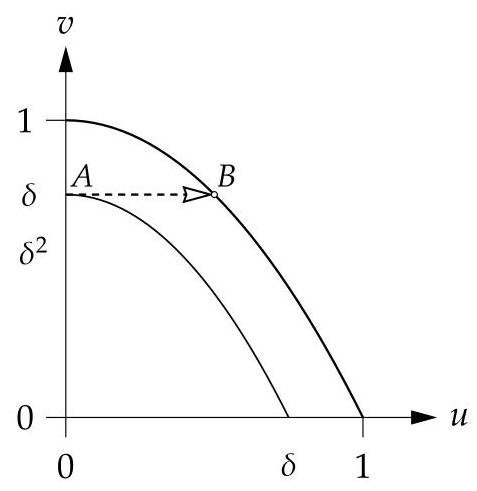
\includegraphics[width=0.3\textwidth]{translation/images/ch11-fig11.jpg}
\caption{图~\ref{fig:11.10}中两轮讨价还价博弈在 \(\delta  = \frac{3}{4}\) 情况下的图解。内侧曲线是第二轮贴现后的收益组合的集合。}
\label{fig:11.11}
\end{figure}

参与人I在首轮提出的分配要求 \(x\)可通过图形法直观求解，具体如图~\ref{fig:11.11} 所示。图中，外侧曲线表示讨价还价集的帕累托前沿，本图采用的是前文使用的效用函数 \(u\left( x\right)  = \sqrt{x}\) 和 \(v\left( y\right)  = y\)。回顾可知，对于 \(0 \leq  x \leq  1\)，可以在该帕累托前沿上得到任意点 \(\left( {u\left( x\right),v\left( {1 - x}\right) }\right)\)。将任意这样的实数对乘以因子 \(\delta\)，就得到了帕累托前沿的“缩小版”，即图中下端点为 \(\left( {\delta ,0}\right)\)、上端点为 \(\left( {0,\delta }\right)\) 的曲线。当 \(y\) 从0变化到1时，观察点 \(\left( {{\delta u}\left( {1 - y}\right),{\delta v}\left( y\right) }\right)\) 就会遍历第二条曲线，这些点是第二轮达成协议后的贴现收益。在由第二轮构成的子博弈中，参与者I只能选择接受或拒绝，因此这个最后通牒博弈的收益组合是曲线的上端点 \(\left( {0,\delta }\right)\)，也就是图~\ref{fig:11.11}中的点 \(A\)。参与者I在第一轮的考虑是在第一轮收益曲线上找到一个点 \(B\)，使得参与者II在接受和拒绝之间无差异（在子博弈完美均衡中她会选择接受）。因此，这个点 \(B\) 与 \(A\) 具有相同的纵坐标 \(\delta\)，即 \(B\) 的形式为 \(\left( {u\left( x\right),\delta }\right)\)。如图中箭头所示，从点 \(A\) 水平移动直到与外曲线相交，就找到了 \(B\)。在这个例子中， \(x\) 是方程\(v\left( {1 - x}\right)  = \delta\)的解，由于 \(v\) 是恒等函数，所以该解就是 \(x = 1 - \delta\)。参与者 \(\mathrm{I}\) 由此获得的效用 \(u\left( x\right)\) 为 \(\sqrt{1 - \delta }\)。图~\ref{fig:11.11}取 \(\delta  = \frac{3}{4}\)进行演示，其中 \(u\left( x\right)  = \frac{1}{2}\) 且 \(v\left( {1 - x}\right)  = \frac{3}{4}\)，即 \(B = \left( {\frac{1}{2},\frac{3}{4}}\right)\)。




\section{多轮交替报价}\label{sec11.9}

三轮交替报价的讨价还价博弈如图~\ref{fig:11.12}所示。参与者I在第一轮提出一个要求 \(x\)，参与者II可以接受或拒绝。如果她拒绝，她可以提出一个反要求 \(y\)，而参与者I又可以接受或拒绝这个反要求。如果参与者I接受，双方的收益都需要进行贴现，得到期望效用对 \(\left( {{\delta u}\left( {1 - y}\right),{\delta v}\left( y\right) }\right)\)。如果参与者I拒绝，那么他可以在第三轮（也就是最后一轮）提出一个二次反要求 \(s\)，如果这个要求被接受，就得到经过两次折现的收益组合 \(\left( {{\delta }^{2}u\left( s\right),{\delta }^{2}v\left( {1 - s}\right) }\right)\)。如果参与者II拒绝最终要求 \(s\)，那么双方收益都为零。这些期望效用之所以会出现，是因为任何一次拒绝都会独立地带来一种风险，即博弈会以概率 \(1 - \delta\)因未达成协议而直接终止，收益为$(0,0)$，并以概率 \(\delta\) 进入下一轮。图~\ref{fig:11.12} 直接展示了经折现后的收益，并未体现议价各轮次间的随机行动；完整模型（如图~\ref{fig:11.10}）才需要把这些随机行动纳入。

\begin{figure}[htbp]
\centering
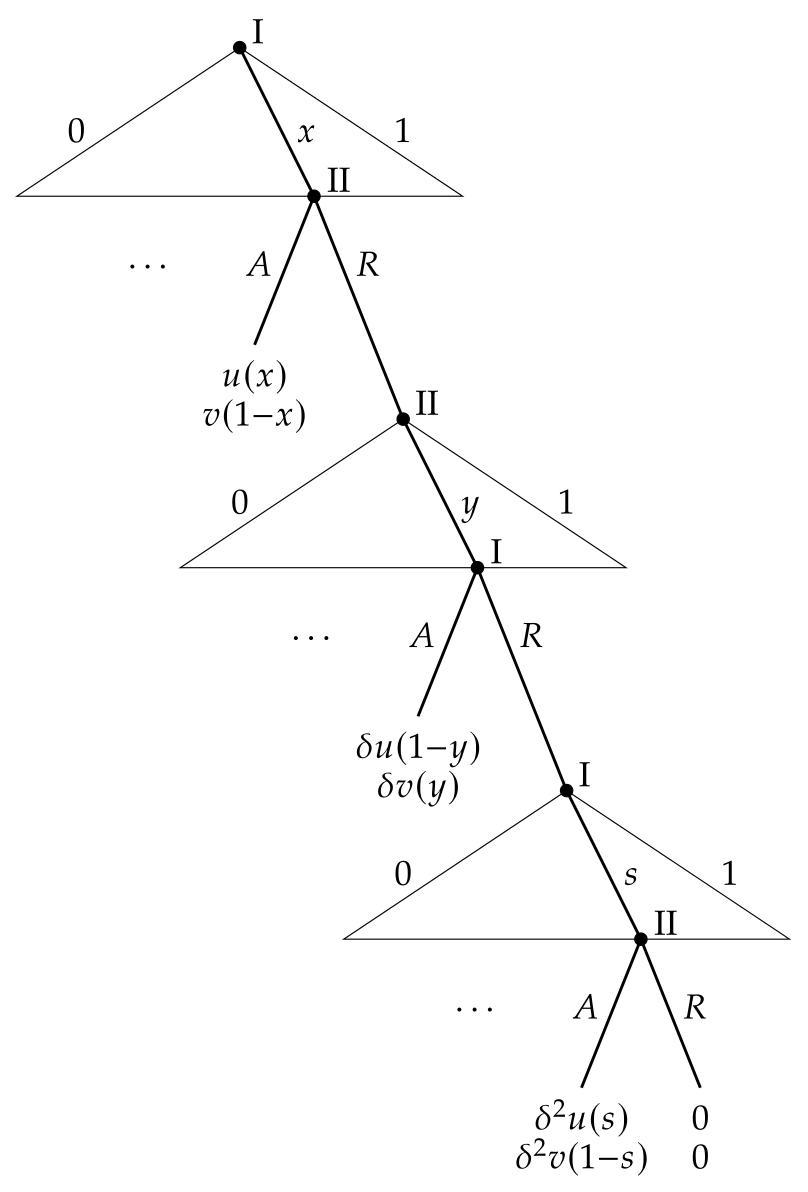
\includegraphics[width=0.6\textwidth]{translation/images/ch11-fig12.jpg}
\caption{三轮讨价还价。}
\label{fig:11.12}
\end{figure}

我们使用逆向归纳法求解该三轮博弈的子博弈完美均衡。第三轮作为最终轮次，是一个由参与者I提出分配要求 \(s = 1\) 参与者II予以接受的最后通牒博弈。经过两次贴现的收益集合 \(\left( {{\delta }^{2}u\left( s\right),{\delta }^{2}v\left( {1 - s}\right) }\right)\) 对应图~\ref{fig:11.13}左侧的内侧曲线。参与者I要求 \(s = 1\)得到收益组合 \(\left( {{\delta }^{2},0}\right)\)，在图中表示为点 \(A\)。在上一轮中，参与者II通过让参与者I在接受和拒绝之间无差异来最大化她的收益 \({\delta v}\left( y\right)\)。

\begin{figure}[htbp]
\centering
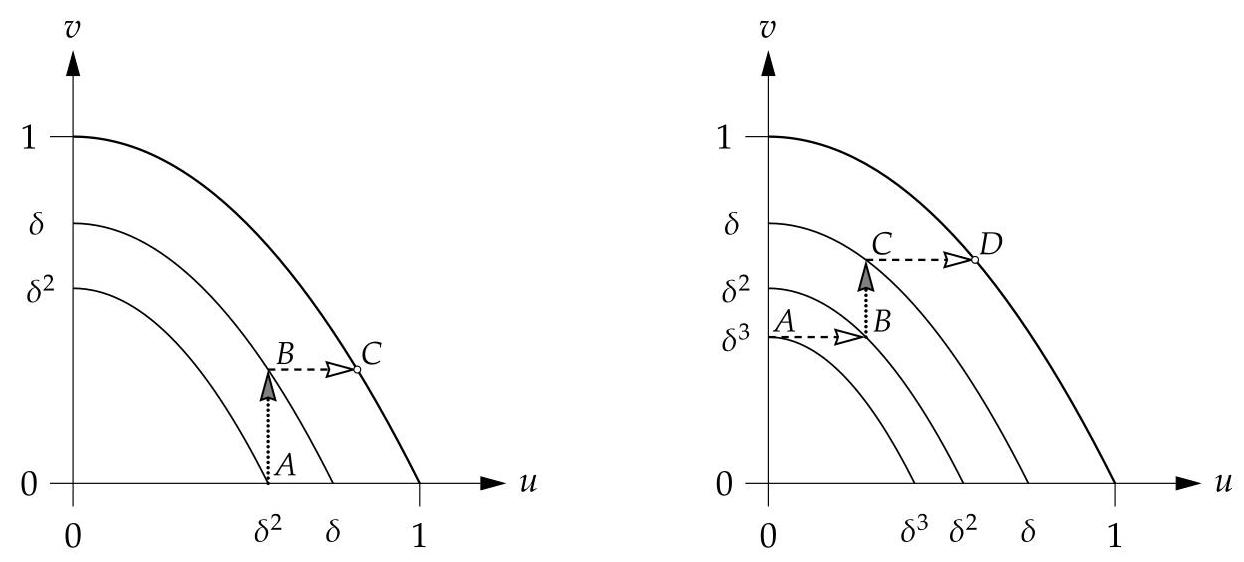
\includegraphics[width=0.9\textwidth]{translation/images/ch11-fig13.jpg}
\caption{三轮（左）和四轮（右）讨价还价博弈的图解。}
\label{fig:11.13}
\end{figure}

因此， \(y\) 是方程 \({\delta u}\left( {1 - y}\right)  = {\delta }^{2}\) 的解，对应图中的点 \(B\)。该点是第二轮收益对曲线 \(\left( {{\delta u}\left( {1 - y}\right),{\delta v}\left( y\right) }\right)\) 上与 \(A\) 具有相同横坐标的点。在这样确定了 \(y\) 之后，参与者I在第一轮的要求 \(x\) 是方程 \(v\left( {1 - x}\right)  = {\delta v}\left( y\right)\) 的解，该条件使得参与者II在第一轮接受和拒绝之间无差异。第一轮收益集合上对应的点 \(C = \left( {u\left( x\right),v\left( {1 - x}\right) }\right)\) 与 \(B\) 具有相同的纵坐标。在均衡路径上，参与者I在第一轮提出要求 \(x\)，参与者II立即接受这个要求。完整的均衡策略和前面的逻辑一致，即参与者会接受所有不超过子博弈完美均衡出价的索取；若对方索取额度超出该水平，则拒绝该提议，并在下一轮提出所述的反要求或二次反要求。

在我们具有效用函数 \(u\left( x\right)  = \sqrt{x}\) 和 \(v\left( y\right)  = y\) 的例子中，根据图~\ref{fig:11.13}中的左图，该三轮博弈的子博弈完美均衡求解如下。从点 \(A\) 到点 \(B\) 的垂直箭头给出方程 \({\delta u}\left( {1 - y}\right)  = {\delta }^{2}\) 即 \(u\left( {1 - y}\right)  = \sqrt{1 - y} = \delta\)，解得 \(y = 1 - {\delta }^{2}\)。从 \(B\) 到 \(C\) 的水平箭头表示方程 \(v\left( {1 - x}\right)  = {\delta v}\left( y\right)\)，即 \(1 - x = \delta \left( {1 - {\delta }^{2}}\right)  = \delta  - {\delta }^{3}\)，其解为 \(x = 1 - \delta  + {\delta }^{3}\)。这就是子博弈完美均衡中玩家I在第一轮的要求；他的收益是 \(u\left( x\right)  = \sqrt{1 - \delta  + {\delta }^{3}}\)。取 \(\delta  = \frac{3}{4}\)，如图~\ref{fig:11.13}所示，我们有 \(y = \frac{7}{16}\) 和 \(x = \frac{43}{64}\)，其中 \(u\left( x\right)  = \sqrt{43}/8\) 且 \(v\left( {1 - x}\right)  = \frac{21}{64}\)。这就是点 \(C\) 的坐标，约为$(0.82, 0.33)$。

四轮讨价还价博弈与三轮博弈结构相同，不同之处在于，如果参与人II在第三轮拒绝了参与人I的需求 \(s\)，她可以在第四轮（即最后一轮）提出自己的最终需求 \(t\)，参与人I只能接受或拒绝。如果参与人I接受，参与人将获得三倍贴现后的收益 \(\left( {{\delta }^{3}u\left( {1 - t}\right),{\delta }^{3}v\left( t\right) }\right)\)。相应的子博弈完美均衡如图~\ref{fig:11.13}右侧所示通过图形求解。最后一轮是一个最后通牒博弈，参与人II可以以 \(t = 1\) 要求得到整个蛋糕，得到收益组合 \(\left( {0,{\delta }^{3}}\right)\)，即图中的点 \(A\)。在前一轮，即博弈的第三轮，参与人 \(\mathrm{I}\) 要求 \(s\)，使得参与人 \(\mathrm{{II}}\) 在接受和拒绝之间效用无差异，得到点 \(B\)，即经过贴现收益组合 \(\left( {{\delta }^{2}u\left( s\right),{\delta }^{2}v\left( {1 - s}\right) }\right)\)，并满足\({\delta }^{2}v\left( {1 - s}\right)  = {\delta }^{3}\)。由此确定\(s\)。再前一轮，参与人II以要求 \(y\) 使参与人I在接受和拒绝之间无差异，满足 \({\delta u}\left( {1 - y}\right)  = {\delta }^{2}u\left( s\right)\)，如图中点 \(C\) 所示。该方程决定了 \(y\)。在第一轮，参与人I根据 \(v\left( {1 - x}\right)  = {\delta v}\left( y\right)\) 要求 \(x\) 以使参与人II无差异，确定点 \(D = \left( {u\left( x\right),v\left( {1 - x}\right) }\right)\)。这也是均衡结果，因为该要求 \(x\) 会被参与人II直接接受。


对于效用函数 \(u\left( x\right)  = \sqrt{x}\) 和 \(v\left( y\right)  = y\)，图~\ref{fig:11.13}中的右图给出了以下子博弈完美均衡。从 \(A\) 到 \(B\) 的箭头给出方程 \({\delta }^{2}v\left( {1 - s}\right)  = {\delta }^{3}\) 即 \(v\left( {1 - s}\right)  = \delta\)，解得参与人I在第三轮的要求 \(s = 1 - \delta\)。从 \(B\) 到 \(C\) 的箭头给出方程 \({\delta u}\left( {1 - y}\right)  = {\delta }^{2}u\left( s\right)\) 或 \(u\left( {1 - y}\right)  = {\delta u}\left( s\right)\)，即 \(\sqrt{1 - y} = \delta \sqrt{1 - \delta }\) 或等价地 \(1 - y = {\delta }^{2}\left( {1 - \delta }\right)  = {\delta }^{2} - {\delta }^{3}\)，其解为 \(y = 1 - {\delta }^{2} + {\delta }^{3}\)，该解确定了参与人II在第二轮的需求 \(y\)。最后，从 \(C\) 到 \(D\) 的箭头给出方程 \(v\left( {1 - x}\right)  = {\delta v}\left( y\right)\) 即 \(1 - x = \delta \left( {1 - {\delta }^{2} + {\delta }^{3}}\right)\)，该方程得出参与人I在第一轮的需求 \(x\) 为 \(x = 1 - \delta  + {\delta }^{3} - {\delta }^{4}\)。

值得注意的是，在四轮讨价还价博弈中，从 \(A\) 到 \(B\) 的箭头所定义的方程与图~\ref{fig:11.11}中的两轮博弈方程完全相同；本质上，四轮博弈的第四轮所描述的情况与两轮博弈的第二轮相同，且图形也一致，唯一区别是所有的收益都缩小了\({\delta }^{2}\)倍。

交替出价的讨价还价博弈可以定义为任意轮数。在每一个奇数轮（第一轮、第三轮、第五轮等），参与人I提出一个要求，参与人II可以接受或拒绝。拒绝后，博弈以概率 \(\delta\) 进入下一轮，否则以收益$(0,0)$结束。参与人II可以在每一个偶数轮提出要求。如果总轮数为偶数，那么参与人II可以提出最后一个需求，即整个蛋糕，这对参与人II有利。如果总轮数为奇数，那么参与人I可以提出最后一个需求，进而为自己要求整个蛋糕。

图~\ref{fig:11.11}和图~\ref{fig:11.13}中的图形解法可以扩展到任意轮数，第 \(k\) 轮的收益为
$(\delta ^{k - 1}u(z),$ $\delta ^{k - 1}v(1 - z))$，其中 \(z \in  \left\lbrack  {0,1}\right\rbrack\)。这些收益组合定义了一条曲线，该曲线是讨价还价集的原始帕累托前沿按照因子\({\delta }^{k - 1}\) 缩放后得到的曲线。两轮、三轮或四轮的例子表明，得到的子博弈完美均衡会确定一个点 \(\left( {u\left( x\right) ,v\left( {1 - x}\right) }\right)\)。这就是两位参与人的收益，因为双方会在第一轮就达成协议。

一般来说，如果总轮数为奇数，参与人I的情况总是好于总轮数为偶数的情况，因为总轮数为偶数有利于能提出最后需求的参与人II。然而，随着总轮数的增加，均衡点 \(\left( {u\left( x\right),v\left( {1 - x}\right) }\right)\) 会相互靠近。我们可以预期，当轮数非常多时，谁能提出最后要求就变得越来越不重要了（因为逆向归纳法所依据的未来贴现期望效用非常小），并且结果会出现某种收敛。不过，我们不会研究这些有限博弈的“极限”，而是考虑一个新概念，即具有无限轮数的博弈。


\section{平稳策略}\label{sec11.10}

我们现在分析具有无限轮数的交替报价讨价还价博弈，也就是说，这个博弈会永远进行下去。形式上，这是一个由无限博弈树表示的具有完美信息的博弈 \(\Gamma\)。其递归结构如图~\ref{fig:11.14}所示。在第一轮和第二轮，参与人I和参与人II分别从区间 \(\left\lbrack  {0,1}\right\rbrack\) 中提出各自的索取份额 \(x\) 和 \(y\)，另一方可以选择接受或者拒绝。若提议遭到拒绝，将触发一个随机行动：博弈会以概率 \(1 - \delta\) 直接终止，此时两名参与人的收益均为零；以概率 \(\delta\) 进入下一轮，此时刚刚拒绝提议的参与人可以提出反索取份额。从第三轮开始，出价权将重新回到参与人I，此时博弈结构与第一轮开局的原博弈 \(\Gamma\) 完全一致。相应地，在参与人I拒绝参与人II的反索取份额 \(y\)、完成第二次随机行动后，后续子博弈的起点就等价于原博弈 \(\Gamma\)。（注：任意一轮索取份额 $x$、后续反索取份额 $y$ 所生成的每一个决策节点处，都会嵌套无穷多个原博弈 $\Gamma$ 的复刻子博弈。）



\begin{figure}[htbp]
\centering
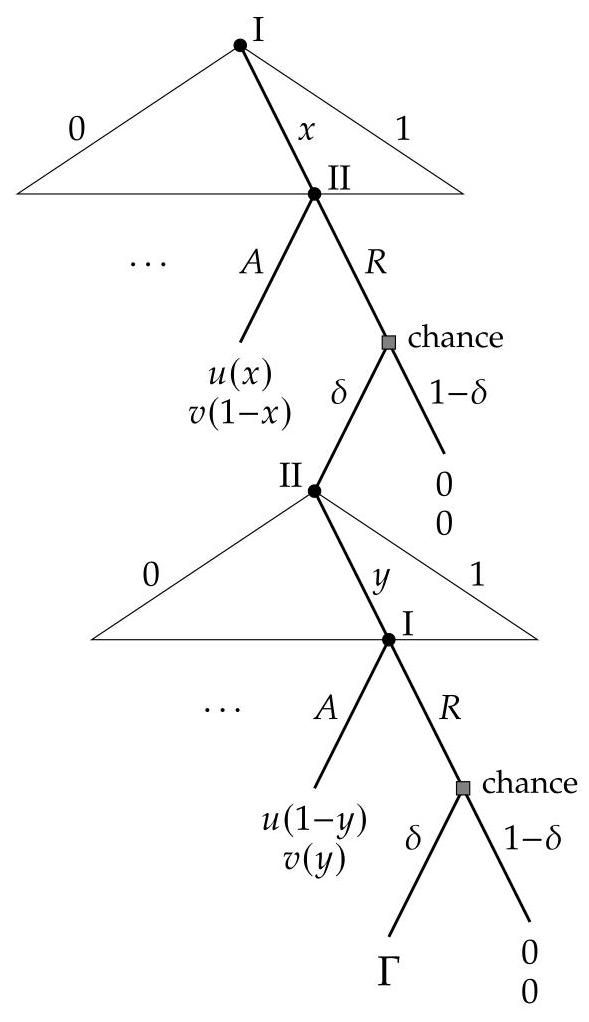
\includegraphics[width=0.4\textwidth]{translation/images/ch11-fig14.jpg}
\caption{具有无限轮数的讨价还价博弈 \(\Gamma\)：在第一轮参与人I提出任意索取份额 \(x\)、第二轮参与人II提出任意索取份额 \(y\)，且双方均拒绝对方的提议之后，该博弈会自我重复。每次以概率 \(\delta\) 进入下一轮，否则以收益 $(0,0)$ 终止。}
\label{fig:11.14}
\end{figure}

这个无限博弈的子博弈完美均衡不能用逆向归纳法来求解，因为博弈会永远进行下去，所以不存在可以作为归纳起点的最终行动。然而，该博弈是递归定义的，经过两轮之后博弈结构保持不变。因此，我们可以定义每两轮重复一次的参与人策略。这样的策略被称为平稳策略：玩家I只要轮到他出价（从第一轮开始的每个奇数轮次）就总是索取份额 \(x\)，而玩家II只要轮到她出价（从第二轮开始的每个偶数轮次）就总是索取份额 \(y\)。子博弈完美均衡条件表明，这些策略应该在该博弈的任何子博弈中定义一个均衡。任何这样的子博弈要么从某一名玩家的索取方案开始，要么从另一名玩家的回应开始，要么从一个随机事件开始。

除了每一轮参与人的索取份额外，子博弈完美均衡还应该规定另一名玩家是接受还是拒绝该提议。一旦提议遭到拒绝，由此产生的期望效用便会乘以贴现因子 \(\delta\) 而缩小。因此，参与人提出的索取份额不能高到令对方选择拒绝，而应当使接受该提议成为对方的最优选择。在满足该条件的前提下，索取份额取到最大值；也就是说，和之前一样，份额的选择要使对方在接受和拒绝之间无差异，并且在子博弈完美均衡中对方会选择接受。

现在我们使用一个类似于图~\ref{fig:11.13}左图的图形来证明子博弈完美均衡的存在性，并说明如何找到它。与该图一样，我们绘制三组收益组合的曲线，它们分别是：如果玩家II接受玩家I在第一轮提出的索取份额 \(x\)，对应的收益组合 \((u(x), v(1 - x))\)；如果玩家I在第二轮接受玩家II的索取份额 \(y\)，对应的贴现收益组合 \((\delta u(1 - y), \delta v(y))\)；如果参与者II在第三轮接受参与者I的索取份额 \(s\)，对应的经过两次贴现的第三轮收益组合 \((\delta^2 u(s), \delta^2 v(1 - s))\)。索取份额 \(x\) 和 \(y\) 的选择要使另一名参与者在接受和拒绝之间无差异。对于第三轮的索取份额 \(s\)，我们希望满足平稳策略的要求，即 \(s = x\)。

图~\ref{fig:11.15}说明了如何满足这些要求。假设玩家I在第三轮的索取份额 \(s\) 对应点 \(A = \left( {{\delta }^{2}u\left( s\right),{\delta }^{2}v\left( {1 - s}\right) }\right)\)，如图~\ref{fig:11.15}(a)所示，该点位于内曲线上相对较高的位置。在前一轮（第二轮），点 \(B = \left( {{\delta u}\left( {1 - y}\right),{\delta v}\left( y\right) }\right)\) 与点 \(A\) 具有相同的横坐标，因为参与者II试图通过她的索取份额 \(y\) 使参与者I在接受和拒绝之间无差异。
\begin{figure}[htbp]
\centering
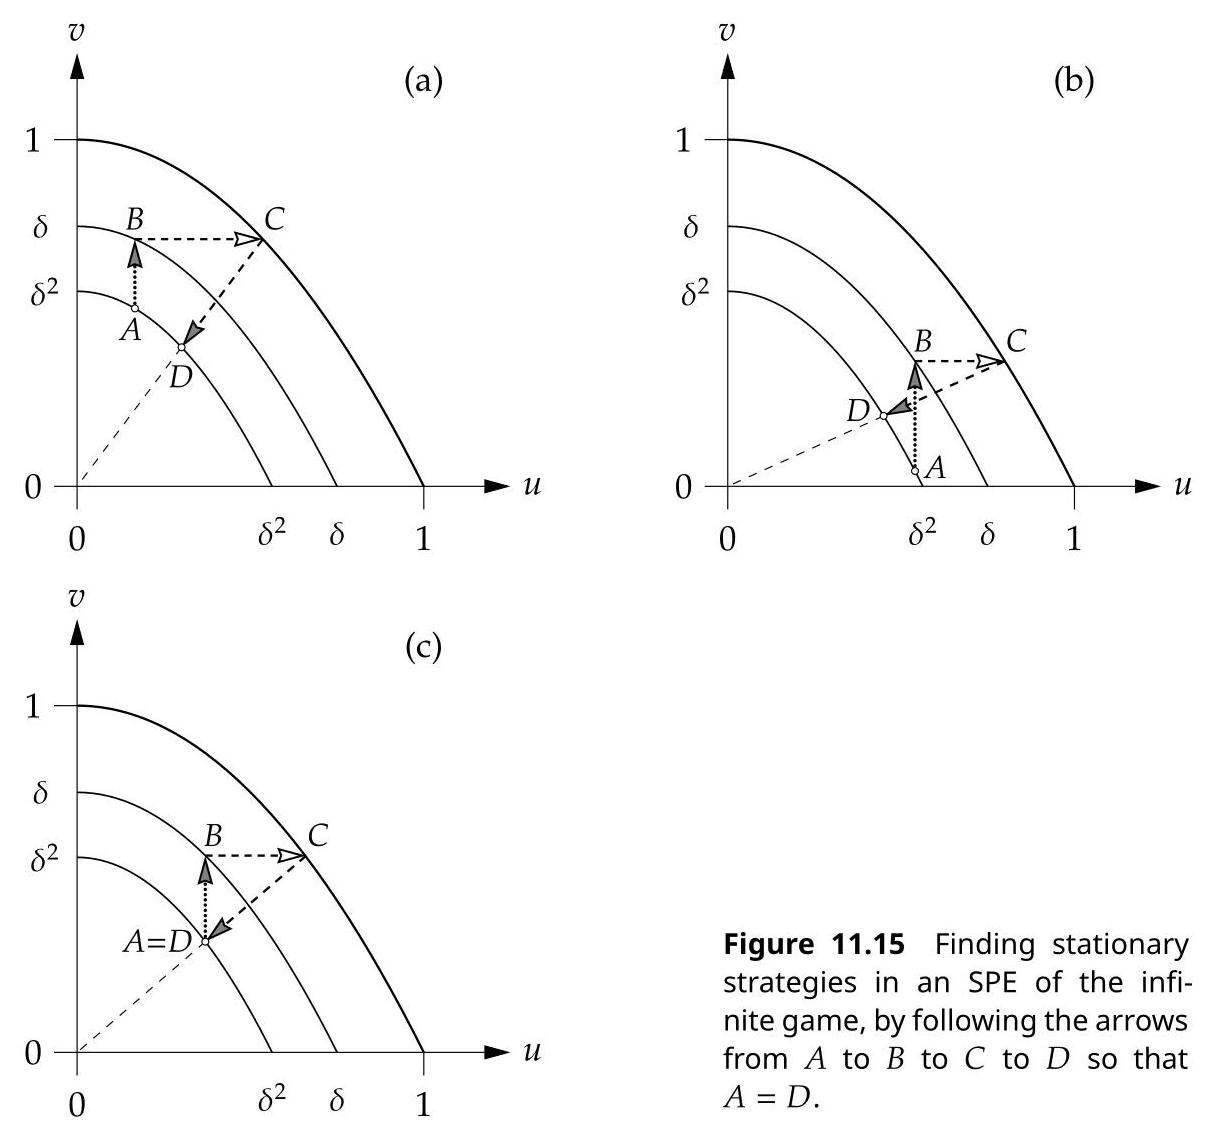
\includegraphics[width=0.9\textwidth]{translation/images/ch11-fig15.jpg}
\caption{寻找无限博弈的子博弈完美均衡中的平稳策略：沿箭头从点 $A$ 到 $B$ 到 $C$ 到 $D$，并使得 $A=D$。}
\label{fig:11.15}
\end{figure}
\begin{equation}
\label{eq:11.4}
{\delta u}\left( {1 - y}\right)  = {\delta }^{2}u\left( s\right)
\end{equation}

在第一轮，用同样的方法得到点 \(C\)，即点 \(\left( {u\left( x\right),v\left( {1 - x}\right) }\right)\)。它与 \(B\) 具有相同的纵坐标，因为参与者I提出索取份额 \(x\)，从而使参与者II在接受和拒绝之间无差异，满足方程：
\begin{equation}
\label{eq:11.5}
v\left( {1 - x}\right)  = {\delta v}\left( y\right)
\end{equation}

如果点 \(C\) 在外部曲线上的相对位置与点 \(A\) 在内曲线上的相对位置相同，那么根据平稳策略的要求，索取份额 \(x\) 与索取份额 \(s\) 相同。在图~\ref{fig:11.15}中，我们将点 \(D\) 定义为 \({\delta }^{2}C\)，即点 \(C\) 按因子 \({\delta }^{2}\) 收缩，代表两轮后的期望收益组合。在图~\ref{fig:11.15}(a)中，点 \(A\) 和 \(D\) 并不重合，因为 \(s < x\)，即第三轮的索取份额 \(s\) 太小。图~\ref{fig:11.15}(b)中的点 \(A\) 对应内曲线上一个对参与者 \(\mathrm{I}\) 过于有利的索取份额 \(s\)；根据方程~\eqref{eq:11.4}和~\eqref{eq:11.5}，从 \(A\) 到 \(B\) 再到 \(C\) 的箭头给出了第一轮索取份额 \(x\)，此时 \(x < s\)。

一般来说，图示说明：从 \(s = 0\) 出发，这些方程给出的第一轮索取份额 \(x\) 满足 \(x > s\)；从 \(s = 1\) 出发，给出的第一轮索取份额 \(x\) 满足 \(x < s\)。此外，从区间 \(\left\lbrack  {0,1}\right\rbrack\) 中任意一个 \(s\) 出发，得到的索取份额 \(x\) 都是 \(s\) 的连续函数。因为连续函数 \(x - s\) 在 \(s = 0\) 处为正，在 \(s = 1\) 处为负，所以一定存在某个中间值 \(s\)，使得 \(s = x\)。这就定义了一个平稳子博弈完美均衡（SPE）。（该子博弈完美均衡也是唯一的，见宾默尔（Binmore，1992，定理 5.8.4）。）

简而言之，无限期讨价还价博弈的平稳子博弈完美均衡是方程组~\eqref{eq:11.4}、\eqref{eq:11.5}和 \(s = x\) 的解。这些方程等价于两个形式优美的对称方程。
\begin{equation}
\label{eq:11.6}
u\left( {1 - y}\right)  = {\delta u}\left( x\right) ,\;v\left( {1 - x}\right)  = {\delta v}\left( y\right).
\end{equation}
第一个方程表示，在每一个偶数轮次中，玩家II通过索取份额 \(y\) 使玩家I在接受与拒绝之间无差异。式~\eqref{eq:11.6}中的第二个方程表示，在每一个奇数轮次中，玩家I通过索取份额 \(x\) 使玩家II在接受与拒绝之间无差异。在这个平稳子博弈完美均衡中，玩家I在第一轮的索取份额 \(x\) 会被玩家II立即接受。和之前一样，完整的策略规定：接受任何更低的索取份额，拒绝任何更高的索取份额。对方实际提出的索取份额总会被接受，因此后续轮次永远不会发生。

在具有效用函数 \(u\left( x\right)  = \sqrt{x}\) 和 \(v\left( y\right)  = y\) 的例子中，子博弈完美均衡中的平稳策略可按如下方式找到。它们由满足方程~\eqref{eq:11.6}的索取份额 \(x\) 和 \(y\) 给出，即

\[
\sqrt{1 - y} = \delta \sqrt{x},\;1 - x = {\delta y}.
\]

第一个方程等价于 \(y = 1 - {\delta }^{2}x\)，将其代入第二个方程得到 \(1 - x = \delta  - {\delta }^{3}x\)，或 \(1 - \delta  = x\left( {1 - {\delta }^{3}}\right)\)。因为 \(1 - {\delta }^{3} = \left( {1 - \delta }\right) \left( {1 + \delta  + {\delta }^{2}}\right)\)，这给出了 \(x\) 和 \(y\) 的解为

\begin{equation}
\label{eq:11.7}
x = \frac{1 - \delta }{1 - {\delta }^{3}} = \frac{1}{1 + \delta  + {\delta }^{2}},\;y = \frac{1 + \delta }{1 + \delta  + {\delta }^{2}}.
\end{equation}

蛋糕在第一轮就完成分配：参与者 I 获得份额 \(x = \frac{1}{1 + \delta  + {\delta }^{2}}\)，参与者 II 获得份额 \(1 - x = \frac{\delta  + {\delta }^{2}}{1 + \delta  + {\delta }^{2}}\)。参与者 II 在第一轮获得的蛋糕份额 \(1 - x\) 低于她在第二轮中的索取份额 \(y\)，如图~\ref{fig:11.15}(c)所示。该图显示外曲线上点 \(A\) 的相对位置高于中间曲线上点 \(B\) 的相对位置，这是因为第二轮的收益经过了贴现。


对于我们的分析来说，由参与者 I 首先提出索取份额是否重要呢？当然，如果改由参与者 II 先提出索取份额，我们只需将两名参与人的身份互换，沿用前文的分析方法即可求解博弈。然而，参与者 II 先行动的博弈及其相应的平稳解，早已蕴含在参与者 I 先行动的原博弈 \(\Gamma\) 的分析框架之内。原因是，参与者 II 先行动的博弈，就是图~\ref{fig:11.14}中参与者 I 先行动的博弈 \(\Gamma\) 在第一次随机行动之后的子博弈，它会像 \(\Gamma\) 中那样重复出现。我们只需忽略参与者 I 的首轮提议、首轮随机行动以及相应的贴现因子 \(\delta\) 即可。也就是说，我们绘制与图~\ref{fig:11.15}中类似的贴现收益对曲线，只是省略外曲线，并将图形乘以 \(\frac{1}{\delta }\) 进行缩放。

对于参与者 II 先行动的交替报价博弈，所得方程仍与前面相同，由式~\eqref{eq:11.6}给出，因此它具有相同的平稳均衡解。这个解从参与者 II 在第一轮索取份额 \(y\) 开始，接着是参与者 I 的反索取份额 \(x\)，后续轮次依此类推。因为在这个子博弈完美均衡中，第一次提出的索取份额会被接受，所以参与者 II 获得收益 \(v\left( y\right)\)，参与者 I 获得收益 \(u\left( {1 - y}\right)\)。根据式~\eqref{eq:11.6}，参与者 I 的收益又等于 \({\delta u}\left( x\right)\)。因此，当参与者 II 先提出索取份额时，唯一的变化是参与者 II 的收益不再乘以 \(\delta\) 进行贴现，而参与者 I 的收益要受到贴现。


\section{交替报价的纳什讨价还价解}\label{sec11.11}

在这最后一节中，我们将证明，当参与者极具耐心、贴现因子 \(\delta\) 无限趋近于 1 时，平稳子博弈完美均衡将会收敛于纳什讨价还价解。我们一直使用的经典例子恰好印证了这一结论：双方具有效用函数 \(u\left( x\right)  = \sqrt{x}\) 和 \(v\left( y\right)  = y\)，其纳什讨价还价解对应的收益分配是 \(\left( {x,1 - x}\right)  = \left( {\frac{1}{3},\frac{2}{3}}\right)\)。该分配也是式~\eqref{eq:11.7}中平稳解在 \(\delta  \rightarrow  1\) 时的极限（注意，表示 \(x\) 的项 \(\frac{1 - \delta }{1 - {\delta }^{3}}\) 中约去了 \(1 - \delta\)；当 \(\delta  = 1\) 时，该式为 \(\frac{0}{0}\) 型未定式，如果不约分，则需要使用洛必达法则求极限）。

\begin{figure}[htbp]
\centering
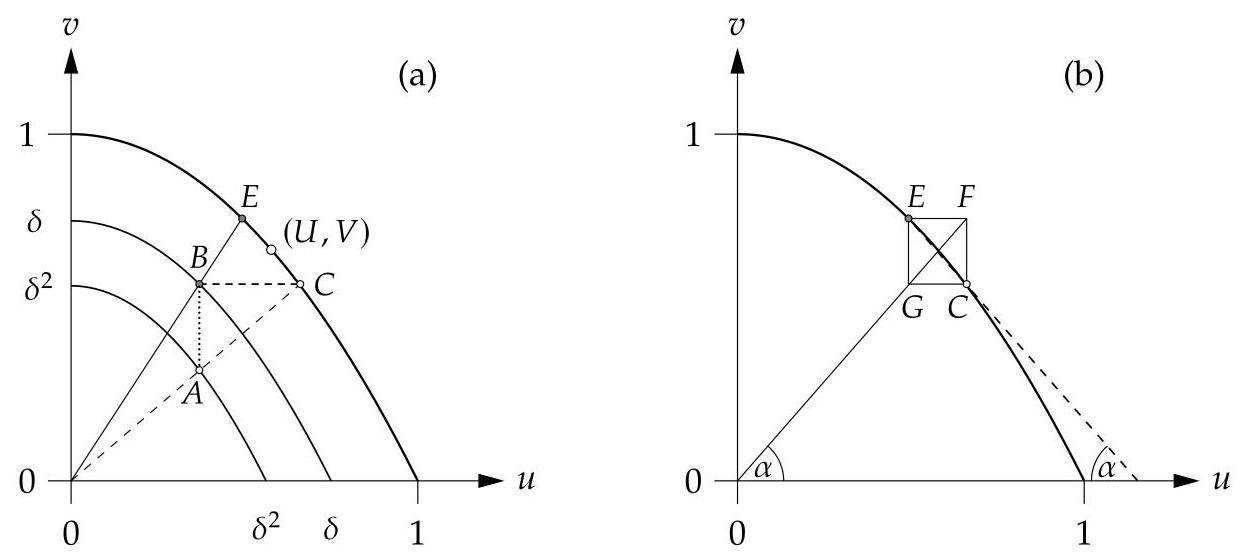
\includegraphics[width=0.9\textwidth]{translation/images/ch11-fig16.jpg}
\caption{为何平稳子博弈完美均衡中参与者的收益会随着
${\color{red}\delta\rightarrow1}$
收敛于纳什讨价还价解 $(U,V)$。点
$C=\left(u(x),v(1-x)\right)$ 是参与者 I 首先提出索取份额时的分配点，
点 $E=\left(u(1-y),v(y)\right)$ 是参与者 II 首先提出索取份额时的分配点。}
\label{fig:11.16}
\end{figure}

交替报价的无限讨价还价博弈的平稳解如图~\ref{fig:11.15}(c)所示，包含点 $B=(\delta u(1-y),$
$\delta v(y))$ 和 \(C = \left( {u\left( x\right),v\left( {1 - x}\right) }\right)\)。上述各点重新标注于图~\ref{fig:11.16}(a)中，并预先标出了纳什讨价还价解 $(U,V)$。定义点 \(E = \left( {u\left( {1 - y}\right),v\left( y\right) }\right)\)，它是点 \(B\) 的“无贴现”形式，即它在外部曲线上的相对位置与 \(B\) 在中间曲线上的相对位置相同。如前一节末尾所述，当参与者II首先提出索取份额 \(y\) 时，该点也是平稳子博弈完美均衡中参与双方的收益。随着 \(\delta  \rightarrow  1\)，点 \(E\) 和 \(C\) 收敛于同一个极限点。如图~\ref{fig:11.16}(b)所示，点 \(E\) 和 \(C\) 确定了一条直线，两点之间的线段是帕累托前沿的一条弦。在极限情况下，这条直线成为帕累托前沿的切线。如果帕累托前沿处处可微，则该切线唯一；即便前沿不可微，取极限后也总能得到前沿的某一条切线。

我们使用图~\ref{fig:11.16}(b)来证明，随着 \(\delta  \rightarrow  1\)，点 \(E\) 和 \(C\) 收敛于纳什讨价还价解。（图中显示，即使当 \(\delta\) 不接近 1 时，\(E\) 和 \(C\) 的中点也已经非常接近 $(U,V)$。）我们使用命题~\ref{prop:11.5}中讨价还价解的几何特征。将点 \(E\) 和 \(C\) 视为一个矩形的左上角和右下角。如图~\ref{fig:11.16}(b)所示，该矩形的右上角是点 \(F = \left( {u\left( x\right),v\left( y\right) }\right)\)，其左下角是点 \(G = \left( {u\left( {1 - y}\right),v\left( {1 - x}\right) }\right)\)。方程~\eqref{eq:11.6}表明 \(G = {\delta F}\)，即点 \(F\) 和 \(G\) 位于一条过原点 $(0,0)$ 的直线上，其中 \(F\) 和 \(G\) 之间的线段是矩形的一条对角线。这条直线的斜率为 \(v\left( y\right) /u\left( x\right)\)，在原点附近表示为角 \(\alpha\)。通过点 \(E\) 和 \(C\) 的矩形的另一条对角线具有绝对值相同、符号相反的斜率，当该直线与 \(u\) 轴相交时表示为角 \(\alpha\)。

在极限情况下，当 \(\delta  \rightarrow  1\) 时，我们有 \(y \rightarrow  1 - x\)，并且得到一个与图~\ref{fig:11.5}中相同的“屋顶”形图形，其两侧的斜率绝对值相同。屋顶的左侧是一条过原点的直线，屋顶的右侧是讨价还价集帕累托前沿的一条斜率与之匹配的切线。这正是命题~\ref{prop:11.5}中把屋顶顶点刻画为纳什讨价还价解 $(U,V)$ 的条件。

我们总结本章的主要结果。具有贴现因子的交替报价模型本身就是一个有趣的非合作博弈。当讨价还价轮数为无限时，该博弈在平稳策略下存在子博弈完美均衡。当贴现因子 \(\delta\) 接近 1 时，这个平稳均衡给出的收益对趋近于纳什讨价还价解。

纳什讨价还价解最初是从讨价还价问题解的合理公理推导出来的。这种解的实现方式在这种公理化方法中并未详细说明，该方法只是假设参与者以某种方式达成了有约束力的协议。

交替报价博弈通过一条完全不同的途径证明了这个解的合理性，即构建参与者不断出价、拒绝出价、反向出价的动态互动模型。在采用平稳策略得到的子博弈完美均衡中，每位参与者都会预判对方后续的行动。双方会立刻达成一致，最终的均衡分配即为纳什讨价还价解。


\section{延伸阅读}\label{sec11.12}

公理化讨价还价模型归功于约翰·纳什（John Nash，1950；不要与纳什均衡混淆）。关于博弈论，特别是合作博弈的权威教科书，是马斯勒（Maschler）、索兰（Solan）和扎米尔（Zamir）于 2013 年合著的著作，其中第 15 章讨论了纳什讨价还价解。奥斯本（Osborne）和鲁宾斯坦（Rubinstein）（1994，第 15 章）以及奥斯本（2004，第 16.3 节）也有相关论述。

支持合作博弈论的观点认为，在实践中，人们遵守协议的假设可能是相当合理的，不必过于担心“执行机制”。荷兰文化史学家约翰·赫伊津哈（Johan Huizinga，1949）认为，“游戏”行为，即出于自身原因愿意遵守相当随意的规则，是文化的一个基本要素；在文化中，即使只是假装遵守游戏规则，也比破坏游戏兴致并质疑游戏本身更容易被容忍。


关于最后通牒博弈的更多细节，请参阅奥斯本（2004，第 6.1.1 节）。具有唯一平稳子博弈完美均衡且趋近于纳什讨价还价解的无限迭代报价讨价还价模型归功于鲁宾斯坦（Rubinstein，1982）。有限多阶段博弈则由斯塔尔（Ståhl，1972）更早提出。

本章的最初灵感来自宾默尔（Binmore，1992，第 5 章）和宾默尔（2007，第 16、17 章）。在那里，假设参与者具有不同的“讨价还价能力”，这反映在参与者不同的贴现因子上。然后，在参与者非常有耐心的无限博弈中，平稳策略趋近于一个“广义”的纳什讨价还价解。我们将其简化为具有相等的讨价还价能力和相等的贴现因子，以便平稳策略趋近于原始的纳什讨价还价解。类似的教科书处理方式可参阅奥斯本（2004，第 16 章）。



\section{第 11 章练习}\label{sec11.13}


\begin{exercise}\label{exer:11.1}
考虑一个威胁点为 $(0,0)$ 的讨价还价集 \(S\)。设 \(a > 0,b > 0\)，且设 \({S}^{\prime } = \{ \left( {{au},{bv}}\right)  \mid  \left( {u,v}\right)  \in  S\}\)。集合 \({S}^{\prime }\) 是 \(S\) 中效用对的集合，参与者 I 的效用按 \(a\) 重新缩放，参与者 II 的效用按 \(b\) 重新缩放。回想一下，讨价还价解的一个公理化性质是：讨价还价结果与这些尺度因子无关。

证明纳什积满足这一性质，即通过最大化纳什积从 \(S\) 得到的纳什讨价还价解重新缩放后成为 \({S}^{\prime }\) 的解。

注意：一旦你能以正确的方式说明“某个量最大化另一个量”的含义，这道题就非常简单。你可能会发现，先考虑更简单的情形 \(b = 1\) 会很有用。
\end{exercise}


\begin{exercise}\label{exer:11.2}

考虑以下两个双矩阵博弈 (i) 和 (ii)：

\begin{center}
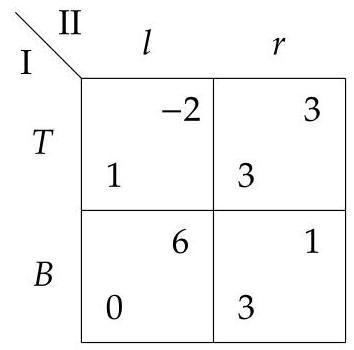
\includegraphics[width=0.2\textwidth]{translation/images/ch11-fig17.jpg}
\end{center}
\hspace*{3em} 

\begin{center}
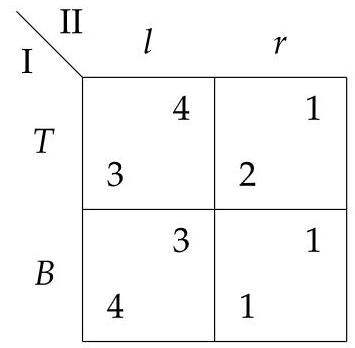
\includegraphics[width=0.2\textwidth]{translation/images/ch11-fig18.jpg}
\end{center}
\hspace*{3em} 

对于每一个双矩阵博弈，完成以下任务：

(a) 分别找出参与者 I 和 II 的极大极小策略 \(\widehat{x}\) 和 \(\widehat{y}\)（可能是混合策略），以及相应的极大极小值 \({u}_{0}\) 和 \({v}_{0}\)。

(b) 绘制 \(2 \times  2\) 博弈中收益对的凸包，以及由满足 \(u \geq  {u}_{0}\) 和 \(v \geq  {v}_{0}\) 的收益对 $(u,v)$ 与 (a) 中找到的威胁点 \(\left( {{u}_{0},{v}_{0}}\right)\) 所构成的讨价还价集 \(S\)。指出 \(S\) 的帕累托前沿。

(c) 求纳什讨价还价解 $(U,V)$。

(d) 说明玩家如何通过在 \(2 \times  2\) 博弈的策略对之间进行联合抽签来实现 \(S\) 的纳什讨价还价解。
\end{exercise}


\begin{exercise}\label{exer:11.3}
我们重新给出离散最后通牒博弈的定义。设 \(M\) 为正整数。玩家 I 的可能行动是提出一个数字 \(x\)，称为他的要求；该数字是 \(0,1,2,\ldots ,M\) 这些整数之一。针对这个要求，玩家 II 可以接受（A）或拒绝（R）。当玩家 II 接受时，玩家 I 获得收益 \(x\)，玩家 II 获得收益 \(M - x\)；当玩家 II 拒绝时，两名玩家的收益均为零。

(a) 当 \(M = 3\) 时，绘制该博弈的博弈树，将其表示为具有完美信息的扩展式博弈。

(b) 对于一般的 \(M\)，玩家 \(\mathrm{I}\) 和玩家 II 分别有多少个纯策略？玩家 I 和玩家 II 在这个博弈中的简化纯策略数量分别是多少？

(c) 求该博弈的所有纯策略子博弈完美均衡。

(d) 求该博弈的所有纯策略均衡（不一定是子博弈完美的）。

(e) 除了 (c) 中的均衡之外，求所有允许双方采用行为策略的子博弈完美均衡。
\end{exercise}




\begin{exercise}\label{exer:11.4}
考虑以下讨价还价问题。通常，一个蛋糕被分割成非负数量的 \(x\) 和 \(y\)，满足 \(x + y \leq  1\)。玩家 \(\mathrm{I}\) 的效用函数是 \(u\left( x\right)  = x\)，玩家 \(\mathrm{{II}}\) 的效用函数是 \(v\left( y\right)  = 1 - {\left( 1 - y\right) }^{2}\)。威胁点是 $(0,0)$。

(a) 绘制讨价还价集（即所有可能的效用对 $(u,v)$ 构成的集合），并在图中指出帕累托前沿。

(b) 求纳什讨价还价解。蛋糕将如何分配？两名玩家的效用分别是多少？
\end{exercise}


\begin{exercise}\label{exer:11.5}
考虑如练习~\ref{exer:11.4}中具有效用函数 \(u,v : \left\lbrack  {0,1}\right\rbrack   \rightarrow  \left\lbrack  {0,1}\right\rbrack\) 的单位蛋糕分配问题，即 \(u\left( x\right)  = x\) 和 \(v\left( y\right)  = 1 - {\left( 1 - y\right) }^{2}\)。现在假设讨价还价行为由具有 \(k\) 轮的标准交替报价讨价还价博弈的子博弈完美均衡描述。在第 1 轮，玩家 I 提出一个特定要求。如果玩家 II 拒绝，她可以在第 2 轮提出一个特定的反要求，后续轮次依此类推。在最后一轮 \(k\)，拒绝意味着两名玩家都得不到任何东西。如果 \(k\) 是奇数，最后提出要求的玩家是玩家 I；如果 \(k\) 是偶数，最后提出要求的玩家是玩家 II。当在第 \(i\) 轮（其中 \(1 \leq  i \leq  k\)）达成协议时，讨价还价集缩小为原来的 \({\delta }^{i - 1}\) 倍。也就是说，每一轮拒绝之后，玩家所能获得的效用都会乘以贴现因子 \(\delta\)。

(a) 假设轮数为 \(k = 2\)。画出这两轮中（对 \(\delta\) 选取某些值）不断缩小的讨价还价集。对于一般的 \(\delta\)，找出子博弈完美均衡，并用参与者 I 的要求 \(x\) 表示。当 \(\delta  = \frac{3}{4}\) 时，要求 \(x\) 是多少？在这个子博弈完美均衡中，两名参与者的策略是什么？


(b) 假设轮数为 \(k = 3\)。画出这三轮中不断缩小的讨价还价集。对于一般的 \(\delta\)，找出子博弈完美均衡，并计算参与者 I 在第一轮提出的要求（你不需要指定参与者的策略）。当 \(\delta  = \frac{1}{4}\) 时，参与者 I 的要求 \(x\) 是多少？（此时 \(x\) 恰好是一个有理数。）


(c) 现在考虑有无穷多轮的情形，并寻找平稳均衡策略，即参与者 I 每次提出要求时都索取相同的份额 \(x\)，参与者 II 每次提出要求时都索取相同的份额 \(y\)。当 \(\delta  = \frac{3}{5}\) 时，要求 \(x\) 是多少？当 \(\delta\) 趋近于 1 时，要求 \(x\) 是多少？将此结果与练习~\ref{exer:11.4}(b)的结果进行比较。
\end{exercise}
